\chapter{极限与函数的连续性}\label{chap:03}

本章讲述数列的极限、具有连续变量的函数的极限以及函数连续的概念．极限的概念与技巧将贯穿全书，本章只是一个引论，以后将逐步深入．因此，在本章中只要求读者对极限在直观了解的基础上，能正确叙述不同变化过程的极限定义，并用于证明极限的四则运算与不等式运算．本章的重要结论之一是，初等函数在它的定义域内都是连续的．

\section{极限问题的提出}\label{sec:3.1}

17 世纪建立的微积分，已有了较为一般的概念，更重要的是提供了一套关于连续变量的崭新的算法，从而成为解决天文、力学、光学与技术问题的重要工具．但那时的微积分，只能说是直观的微积分．因为它的一些基本概念并不确切，甚至逻辑推导前后矛盾．例如，微积分的一个最重要的概念——微商，它反映了一个连续量对另一个连续量的``瞬时变化率''，其概念就很不确切，逻辑推导前后矛盾．牛顿当时把连续量称为流量，把变化率称为流数（把自变量理解为时间）．例如把自由落体的路程看作流量，流数就是瞬时速度．用今天的符号，牛顿当时推导流数的方法是：对自由落体的运动规律 $s = \frac{1}{2}gt^2$，给时间 $t$ 一个微小的改变 $h$（他称之为瞬——moment），则平均速度为
\[
\frac{\frac{1}{2}g(t+h)^2-\frac{1}{2}gt^2}{h} = gt + \frac{1}{2}gh.
\]
然后令 $h=0$，便得瞬时速度 $gt$．凭着类似的推导，微积分的演算系统建立起来了．但这里的瞬 $h$ 究竟是什么？贝克莱（Berkeley，1685---1753）就曾指出这里有逻辑错误．因为在计算平均速度时，要用 $h$ 去除，必须假设 $h \neq 0$．但为最后得到瞬时速度，必须令 $h=0$，才能算出 $gt$．$h$ 非零又是零，$h$ 到底是什么？难怪贝克莱讥讽说这是``消失的量的鬼魂''．这个问题困惑了数学家很长时间．达朗贝尔认为说清楚这点，应该用极限，但他并没有把它说清楚．拉格朗日企图用代数推演的方法逃避这个困难，但这脱离了微积分的物理意义，很难应用．直到 19 世纪柯西才真正用极限的概念把它基本说清楚，而魏尔斯特拉斯最终用 $\varepsilon - \delta$ 的语言，彻底解决了这个困难，从而推动了近代分析的蓬勃发展．

极限最早的观念，在国外有所谓``穷竭法''，在中国有所谓割圆术，即把圆近似地割成边数很多、边长很细的正多边形来计算圆面积．魏晋时代的刘徽就说过：``割之弥细，所失弥小，割之又割，以至于不可割，则与圆周合体而无所失矣''．后来，和微积分同时产生而用得很多的一种运算，就是无穷多项相加
\[
a_1 + a_2 + \cdots + a_n + \cdots.
\]
怎样理解这无穷多项相加？这只能理解为有限项相加，但越加越多，最后看它的变化趋势，这就是所谓的数列极限．把数列极限的思想用来观察求瞬时速度的推导，就是把 $h$ 看成越变越小而且无限地变小（但不为零），来研究平均速度的变化趋势，从而建立一套从平均速度求瞬时速度的计算方法，这就是所谓的函数极限．今天，我们学习微积分，当然不必重复历史的过程，而可以从严格的极限概念开始，严格地讲述微积分的概念、演算及应用．

下面我们先从数列极限入手，然后讲述函数极限，再用函数极限，给出函数连续的概念，并最后证明，一切初等函数在其定义域是连续的．从下一章开始转入微积分．

\section{数列的极限}\label{sec:3.2}

\begin{definition}\label{def:3-1}
定义域为正整数的函数称为数列，记为 $\{x_n\}$．即有 $x_n = f(n)$，$n \in \mathbb{N}_+$．
\end{definition}

$x_n$ 是数列的第 $n$ 项，表示函数在 $n$ 处的函数值，而 $\{x_n\}$ 则表示数列．由于正整数有自然的顺序，故数列也可以写成
\[
x_1, x_2, x_3, \cdots, x_n, \cdots.
\]
这也是数列的一种表示．

$x_n$ 也叫做数列的通项，我们经常可以通过给出第 $n$ 项 $x_n$ 的显式来给出一个数列．

例如 $x_n = \frac{1}{n}$，写出来就是 $1, \frac{1}{2}, \frac{1}{3}, \frac{1}{4}, \cdots$；

$x_n = \frac{(-1)^n}{n}$，写出来就是 $-1, \frac{1}{2}, -\frac{1}{3}, \frac{1}{4}, \cdots$；

$x_n = \frac{n+1}{n}$，写出来就是 $2, \frac{3}{2}, \frac{4}{3}, \frac{5}{4}, \cdots$；

$x_n = n^2$，写出来就是 $1, 4, 9, 16, \cdots$；

$x_n = 1+(-1)^n$，写出来就是 $0, 2, 0, 2, \cdots$．

也有些数列的通项不能用显式表示出来．

例如，$c$ 是无理数，它可用无限不循环小数表示
\[
c_0.c_1c_2\cdots c_n\cdots.
\]
令 $x_n = c_0.c_1c_2\cdots c_n$，这样定义的数列 $\{x_n\}$，一般说来，它的通项不能用显式表示出来．

数列也可以用递推的方法给出，例如，$a_0 = 0$，$a_1 = 1$，$a_{n+1} = \frac{a_{n-1}+a_n}{2}$，$n=1,2,\cdots$ 就定义一个数列，它的前六项是
\[
0, 1, \frac{1}{2}, \frac{3}{4}, \frac{5}{8}, \frac{11}{16}.
\]

\subsection*{1. 极限的概念}

根据§\ref{sec:3.1}问题的提出，我们要研究数列的极限，就是看当 $n$ 无限增大时，$x_n$ 的变化趋势如何．换句话说，看是否存在一个常数 $a$，当 $n$ 无限增大时，$x_n$ 的值无限地接近 $a$．在回答是肯定的情形下，就可以说 $\{x_n\}$ 的极限是 $a$．

我们来看前面提出的几个例子．

\begin{example}\label{ex:3-2-1}
$x_n = \frac{1}{n}$．容易看出，当 $n$ 无限增大时，$x_n$ 无限接近于 $0$，因而 $x_n$ 的极限为 $0$．
\end{example}

\begin{example}\label{ex:3-2-2}
$x_n = \frac{(-1)^n}{n}$．当 $n$ 无限增大时，它的值时而为正，时而为负，但总的趋势仍然是无限地接近于 $0$ 这个数，因此 $x_n$ 的极限也是 $0$．
\end{example}

\begin{example}\label{ex:3-2-3}
$x_n = \frac{n+1}{n}$，即
\[
2, \frac{3}{2}, \frac{4}{3}, \frac{5}{4}, \cdots, \frac{101}{100}, \frac{102}{101}, \cdots,
\]
当 $n$ 无限增大时，$x_n$ 越变越小，无限地接近于 $1$，因此 $x_n$ 的极限是 $1$．
\end{example}

\begin{example}\label{ex:3-2-4}
$x_n = n^2$．当 $n$ 无限增大时，$n^2$ 也无限增大，并不无限接近一个常数，因此说它没有极限．
\end{example}

\begin{example}\label{ex:3-2-5}
$x_n = 1+(-1)^n$．它在 $0$ 与 $2$ 两个数中不停地跳动，也不是无限地接近一个常数，因此也没有极限．
\end{example}

现在我们可以来分析一下，一般地说，当 $n$ 无限增大时，$x_n$ 无限接近于 $a$，确切的意思究竟是什么？

两个数接近的程度可以用它们的差的绝对值（在数轴上，就是这两个点之间的距离）来衡量．因此，以 $x_n = \frac{1}{n}$ 为例，说 $x_n$ 与 $0$ 很接近，即是说 $x_n$ 与 $0$ 的距离 $|x_n - 0|$ 很小．例如
\[
\text{当 } n>2 \text{ 时},\quad |x_n - 0| = \frac{1}{n} < \frac{1}{2},
\]
当 $n>3$ 时，$|x_n - 0| = \frac{1}{n} < \frac{1}{3}$，

当 $n>N$ 时，$|x_n - 0| = \frac{1}{n} < \frac{1}{N}$．

上面左边一列是 $n$ 增大的程度．相应地，右边一列是 $x_n$ 与 $0$ 的接近程度．$n$ 增大的程度不同，则 $x_n$ 与 $0$ 的接近程度也不同．$n$ 只要大到比 $N$ 大，就可以保证 $x_n$ 与 $0$ 的距离小于 $\frac{1}{N}$．直观形象地说，如果把数列
\[
x_1, x_2, \cdots, x_N, x_{N+1}, x_{N+2}, \cdots
\]
从第 $N+1$ 项起后面的所有项叫做数列 $\{x_n\}$ 的尾巴，则尾巴中的每项与 $0$ 的距离都小于 $\frac{1}{N}$．

我们已经看到，对于足够大的 $N$ 之后的所有 $n$，可以使 $|x_n - 0|$ 小到一定程度，但还不能说明 $|x_n - 0|$ 无限小．如何反映``无限''二字呢？我们说当 $n$ 无限增大时，$x_n$ 无限接近于 $0$，即是说 $x_n$ 与 $0$ 的距离 $|x_n - 0|$ 可以任意小，只要 $n$ 足够大（$n > N$）．可见``无限''能用距离的任意性来反映，即对于任意的正数 $\varepsilon$，不论它多么小，只要 $N$ 足够大，对于所有的 $n > N$，都能保证 $|x_n - 0| < \varepsilon$．事实上，要使
\[
|x_n - 0| = \frac{1}{n} < \varepsilon,
\]
只要 $n > \frac{1}{\varepsilon}$．故取 $N = \left[\frac{1}{\varepsilon}\right]$，则对大于 $N$ 的所有正整数 $n$，上式总成立．

将上面的语言抽象化，便有下面的定义．

\begin{definition}\label{def:3-2}
设 $\{x_n\}$ 是一数列，$a$ 是一实数．若对于任意给定的正数 $\varepsilon$，存在正整数 $N$，当 $n > N$ 时，都有
\[
|x_n - a| < \varepsilon,
\]
则称 $a$ 是数列 $\{x_n\}$ 当 $n$ 趋于无穷时的极限，或称数列 $\{x_n\}$ 收敛，且收敛于 $a$，记为
\[
\lim_{n\to\infty}x_n = a,\qquad \text{或}\qquad x_n \to a\quad(n\to\infty).
\]
没有极限的数列称为发散数列．
\end{definition}

从几何上看，数列 $\{x_n\}$ 的极限为 $a$，是指任意给定以 $a$ 为中心的区间 $(a-\varepsilon, a+\varepsilon)$，必然从某项 $x_{N+1}$ 起，后面的所有项都落在区间 $(a-\varepsilon, a+\varepsilon)$ 之中．换句话说，数列 $\{x_n\}$ 至多有 $N$ 项 $x_1, x_2, \cdots, x_N$ 落在区间 $(a-\varepsilon, a+\varepsilon)$ 之外（见图~\ref{fig:3-1}）．这就是数列极限的几何意义．由此也可以看出，数列的前有限项并不影响数列的收敛性和极限．即添加或修改数列的有限项，并不影响数列的收敛性与极限．

\begin{figure}[htbp]
\centering
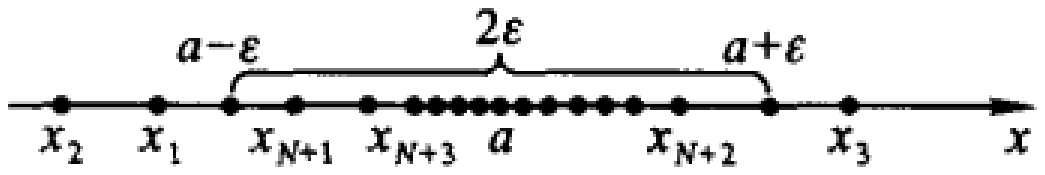
\includegraphics[width=0.72\textwidth]{work/figures/fig3-1}
\figcap\label{fig:3-1}
\end{figure}

定义中描述数列极限的语言称为 $\varepsilon - N$ 语言．正数 $\varepsilon$ 用来反映 $x_n$ 与 $a$ 的接近程度，而 $\varepsilon$ 的任意性就反映了 $x_n$ 与 $a$ 可以任意接近，或说无限接近．$\varepsilon$ 是任意的，也是相对固定的．对每一个固定的 $\varepsilon > 0$，相应地有一个 $N$，$N$ 是随 $\varepsilon$ 的变化而变化的．一般地说，$\varepsilon$ 越小则 $N$ 越大．$N$ 一旦存在则不是唯一的，不过重要的是 $N$ 的存在性，而不是 $N$ 取什么值．

\begin{definition}\label{def:3-3}
极限为 $0$ 的数列称为无穷小量．
\end{definition}

值得注意的是无穷小量是一数列，而不是一个很小的常数．由极限定义显然有，$\{x_n\}$ 以 $a$ 为极限等价于数列 $\{x_n - a\}$ 以 $0$ 为极限．我们把它写成下面的命题．

\begin{proposition}\label{prop:3-1}
$\{x_n\}$ 的极限为 $a$ 的充要条件是 $\{x_n - a\}$ 是无穷小量．
\end{proposition}

数列极限定义本身并没有给出求极限的方法，但它却深刻地描述了数列趋向极限的变化过程．当估计出数列的极限后，可以用定义来验证估计的正确性．下面举例说明．

\begin{example}\label{ex:3-2-6}
证明 $\lim_{n\to\infty}\frac{1}{n^p} = 0$ ($p>0$)．
\end{example}

\begin{proof}
对任意给定的 $\varepsilon>0$，要使
\[
\left|\frac{1}{n^p} - 0\right| = \frac{1}{n^p} < \varepsilon,
\]
只要 $n > \left(\frac{1}{\varepsilon}\right)^{\frac{1}{p}}$．取 $N = \left[\left(\frac{1}{\varepsilon}\right)^{\frac{1}{p}}\right] + 1$，则当 $n > N$ 时，有
\[
\left|\frac{1}{n^p} - 0\right| < \varepsilon.
\]
故 $\left\{\frac{1}{n^p}\right\}$ 的极限为 $0$．
\end{proof}

\begin{example}\label{ex:3-2-7}
设 $|q|<1$，证明 $\lim_{n\to\infty}q^n = 0$．
\end{example}

\begin{proof}[证法 1]
若 $q = 0$，结论显然成立．故不妨设 $q \neq 0$．对任意给定的 $\varepsilon > 0$，不妨设 $\varepsilon < 1$，要使
\[
|q^n - 0| = |q^n| < \varepsilon,
\]
即
\[
n\lg|q| < \lg\varepsilon,
\]
只要
\[
n > \frac{\lg\varepsilon}{\lg|q|}.
\]
令 $N = \left[\frac{\lg\varepsilon}{\lg|q|}\right] + 1$，则当 $n > N$ 时，有 $|q^n| < \varepsilon$．这就证明了 $\lim_{n \to \infty} q^n = 0$．
\end{proof}

\begin{proof}[证法 2]
不妨设 $q \neq 0$．由 $|q| < 1$ 知存在 $\alpha > 0$，使得 $|q| = \frac{1}{1 + \alpha}$，从而
\[
|q|^n = \frac{1}{(1 + \alpha)^n} = \frac{1}{1 + n\alpha + \cdots + \alpha^n} < \frac{1}{n\alpha}.
\]
对任给的 $\varepsilon > 0$，要使 $|q^n| < \varepsilon$，只要放大后的 $\frac{1}{n\alpha} < \varepsilon$．因此取 $N = \left[\frac{1}{\alpha\varepsilon}\right] + 1$，则当 $n > N$ 时，有
\[
|q^n - 0| = |q|^n < \frac{1}{n\alpha} < \varepsilon.
\]
这就证明了 $\lim_{n\to\infty}q^n = 0$．
\end{proof}

从前面的例子可见，整个证明过程实际上是找 $N$ 的过程，采用的是反推法，即从 $|x_n - a| < \varepsilon$ 出发，看满足条件的 $N$ 是否存在．我们只要找到一个就可以了，不管用的是什么方法．证法 2 用的是适当放大法，它将 $|q^n - 0|$ 适当放大到 $\frac{1}{n\alpha}$，使我们很容易找到 $N$．当然放大要适当，要保证把 $|x_n - a|$ 放大以后仍然是无穷小量．下面再举几个适当放大的例子．

\begin{example}\label{ex:3-2-8}
设 $a > 0$，证明 $\lim_{n \to \infty} \sqrt[n]{a} = 1$．
\end{example}

\begin{proof}
若 $a=1$，结论显然成立．

设 $a > 1$．记 $\sqrt[n]{a} = 1 + \alpha_n$ ($\alpha_n > 0$)，则
\[
a = (1 + \alpha_n)^n = 1 + n\alpha_n + \cdots + \alpha_n^n > n\alpha_n.
\]
因此
\[
|\sqrt[n]{a} - 1| = \alpha_n < \frac{a}{n}.
\]
对任意给定的 $\varepsilon>0$，不妨设 $\varepsilon<1$，取 $N = \left[\frac{a}{\varepsilon}\right]$，则当 $n>N$ 时，有
\[
|\sqrt[n]{a} - 1| < \frac{a}{n} < \varepsilon.
\]
最后设 $0 < a < 1$．这时存在 $b > 1$ 使 $a = \frac{1}{b}$，因此
\[
|\sqrt[n]{a} - 1| = \left|\sqrt[n]{\frac{1}{b}} - 1\right| = \frac{|1 - \sqrt[n]{b}|}{\sqrt[n]{b}} < |1 - \sqrt[n]{b}|.
\]
由于 $\lim_{n\to\infty}\sqrt[n]{b} = 1$，故对任给 $\varepsilon>0$，存在 $N$，当 $n>N$ 时，有
\[
|\sqrt[n]{a} - 1| < |1 - \sqrt[n]{b}| < \varepsilon.
\]
这样，我们证明了当 $a > 0$ 时，总有 $\lim_{n \to \infty} \sqrt[n]{a} = 1$．
\end{proof}

\begin{example}\label{ex:3-2-9}
证明 $\lim_{n\to\infty}\frac{n^2+1}{n^2-n-2} = 1$．
\end{example}

\begin{proof}
当 $n>4$ 时，
\[
\left|\frac{n^2+1}{n^2-n-2} - 1\right| = \left|\frac{n+3}{n^2-n-2}\right| = \frac{n+3}{n^2-n-2} < \frac{2n}{n^2 - \frac{n^2}{4} - \frac{n^2}{4}} = \frac{4}{n}.
\]
对任给的 $\varepsilon>0$，取 $N = \max\left(4, \left[\frac{4}{\varepsilon}\right]\right)$，则当 $n>N$ 时，有
\[
\left|\frac{n^2+1}{n^2-n-2} - 1\right| < \frac{4}{n} < \varepsilon,
\]
即
\[
\lim_{n\to\infty}\frac{n^2+1}{n^2-n-2} = 1.
\]
\end{proof}

研究数列的极限，就是要从数列出发，把它的极限求出来．可见从数列到极限，也是一种运算，但它同第一章讲数系时的运算很不同．那时是从两个数（或有穷个数）出发求一个数，例如从 $a$ 和 $b$ 求 $a+b$．求极限则完全不同了，是从一个数列，即从无穷个数出发，求一个数．从无穷个数到一个数，这就是极限运算的特点．正是由于这个特点，使极限的计算变得十分复杂．因此，人们需要有一个一般的准则来检验计算是否正确．当然，这个准则不仅在检验一些具体数列的极限时是重要的，而更重要的是它对理论上的推理是必不可少的．这个准则就是极限的 $\varepsilon-N$ 定义，它是人类经过漫长的时间才抽象出来的．我们并不要求读者立刻全面地理解，只希望读者在今后的学习过程中，通过大量的反复的应用逐步地掌握它．

\subsection*{2. 极限与四则运算及与不等式的关系}

下面我们要来寻找求极限的方法．

回忆学算术的过程，我们可以计算任何两个数的乘法．为什么呢？实际上，我们所掌握的，一是九九表，二是一套进位规则（当然还包括小数点的计算）．何谓进位规则？其实说的是加法与乘法的分配律，也就是加法与乘法的运算次序可以交换：
\[
a(b+c) = ab + ac.
\]
例如，$26 \times 8 = 208$，是这样计算出来的：
\[
\begin{array}{r}
2\ 6 \\
\times \quad 8 \\
\hline
4\ 8 \\
1\ 6\ 0 \\
\hline
2\ 0\ 8
\end{array}
\]
实际上根据的就是加法与乘法可以交换次序：
\[
26\times8 = (20+6)\times8 = 20\times8 + 6\times8 = 160 + 48 = 208.
\]
因此，我们希望能学会求更多数列的极限，自然就会问，对极限这一新的运算，它和别的运算间是否也有类似的规律？事实上，并非所有的运算都具有类似的性质．例如等式
\[
\sqrt{a+b} = \sqrt{a} + \sqrt{b}
\]
就不是永远成立的，即开平方运算与加法运算并不能交换次序．若能设想这等式成立，开平方运算就会变得简单得多了．

极限是对无穷个数进行的运算，它和四则运算的次序能否交换？幸好，回答是肯定的．当然，这是需要证明的，因为极限运算是一种崭新的运算．

\begin{theorem}\label{thm:3-1}
设 $\lim_{n\to\infty}x_n = a$，$\lim_{n\to\infty}y_n = b$，则
\begin{enumerate}[label=\roman*)]
\item $\lim_{n\to\infty}(x_n \pm y_n) = a \pm b$；
\item $\lim_{n \to \infty} (x_n y_n) = ab$；
\item $\lim_{n \to \infty} \frac{x_n}{y_n} = \frac{a}{b} \quad (b \neq 0)$．
\end{enumerate}
\end{theorem}

定理~\ref{thm:3-1} 表明两数列对应项的代数和（积、商）的极限等于极限的代数和（积、商），因此实际上说的是极限运算和四则运算次序是可以交换的．我们可以把定理~\ref{thm:3-1} 写成
\[
\lim_{n\to\infty}(x_n \pm y_n) = \lim_{n\to\infty}x_n \pm \lim_{n\to\infty}y_n;
\]
\[
\lim_{n\to\infty}(x_n y_n) = \lim_{n\to\infty}x_n \cdot \lim_{n\to\infty}y_n;
\]
\[
\lim_{n\to\infty}\frac{x_n}{y_n} = \frac{\lim\limits_{n\to\infty}x_n}{\lim\limits_{n\to\infty}y_n}\qquad \left(\text{当 }\lim_{n\to\infty}y_n \neq 0\right).
\]
值得注意的是，其前提是等式右边的极限都事先假设是存在的．

为了证明 ii)，我们将要用到收敛数列的有界性．为了证明 iii)，又要用到极限的保号性．因此，我们先给出这两个性质，再回头来证明定理~\ref{thm:3-1}．

回忆函数的有界性定义，知数列 $\{x_n\}$ 有界是指存在正数 $M$，使得
\[
|x_n| \leqslant M
\]
对一切 $n$ 成立．

\begin{theorem}[有界性]\label{thm:3-2}
有极限存在的数列必有界．
\end{theorem}

\begin{proof}
设数列 $\{x_n\}$ 有极限 $a$．由极限定义，对 $\varepsilon_0 = 1$，则存在 $N$，当 $n>N$ 时，有
\[
|x_n - a| < 1.
\]
因此
\[
|x_n| = |x_n - a + a| \leqslant |x_n - a| + |a| < 1 + |a|.
\]
令 $M = \max(|x_1|, |x_2|, \cdots, |x_N|, 1+|a|)$，则
\[
|x_n| \leqslant M,\qquad n=1,2,\cdots.
\]
这就证明了 $\{x_n\}$ 是有界的．
\end{proof}

\begin{corollary}\label{cor:3-1}
若 $\{x_n\}$ 无界，则 $\{x_n\}$ 发散．
\end{corollary}

\begin{theorem}[保号性]\label{thm:3-3}
若 $\lim_{n\to\infty}x_n = a$，$a>0$，则存在 $N$，当 $n>N$ 时，有 $x_n > \frac{a}{2} > 0$．
\end{theorem}

\begin{proof}
由 $\lim_{n\to\infty}x_n = a > 0$，知对 $\varepsilon_0 = \frac{a}{2} > 0$，存在 $N$，当 $n>N$ 时，有
\[
|x_n - a| < \frac{a}{2},
\]
从而
\[
x_n > a - \frac{a}{2} = \frac{a}{2} > 0.
\]
定理证完（见图~\ref{fig:3-2}）．
\end{proof}

\begin{figure}[htbp]
\centering
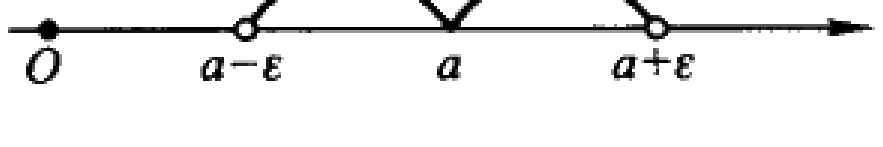
\includegraphics[width=0.48\textwidth]{work/figures/fig3-2}
\figcap\label{fig:3-2}
\end{figure}

\begin{corollary}\label{cor:3-2}
设 $\lim_{n\to\infty}x_n = a$．
\begin{enumerate}[label=\roman*)]
\item 若 $a<0$，则存在 $N$，当 $n>N$ 时，有 $x_n < \frac{a}{2} < 0$；
\item 若 $a \neq 0$，则存在 $N$，当 $n > N$ 时，有 $|x_n| > \frac{|a|}{2} > 0$．
\end{enumerate}
\end{corollary}

请读者写出推论~\ref{cor:3-2} 的证明．

\begin{proof}[定理~\ref{thm:3-1} 的证明]
i) 对任意给定的 $\varepsilon>0$，由 $\lim_{n\to\infty} x_n = a$，存在 $N_1$，当 $n>N_1$ 时，有
\[
|x_n - a| < \frac{\varepsilon}{2}.
\]
由 $\lim_{n\to\infty}y_n = b$，知存在 $N_2$，当 $n>N_2$ 时，有
\[
|y_n - b| < \frac{\varepsilon}{2}.
\]
取 $N = \max(N_1, N_2)$，则当 $n > N$ 时，有
\[
|x_n \pm y_n - (a \pm b)| \leqslant |x_n - a| + |y_n - b| < \frac{\varepsilon}{2} + \frac{\varepsilon}{2} = \varepsilon,
\]
即
\[
\lim_{n\to\infty}(x_n \pm y_n) = a \pm b.
\]

ii) 对任意 $n$，有
\[
\begin{aligned}
|x_n y_n - ab| &= |x_n y_n - x_n b + x_n b - ab| \\
&\leqslant |x_n y_n - x_n b| + |x_n b - ab| \\
&= |x_n||y_n - b| + |b||x_n - a|.
\end{aligned}
\]
任给 $\varepsilon>0$，由 $\lim_{n\to\infty}x_n = a$ 与 $\lim_{n\to\infty}y_n = b$，以及定理~\ref{thm:3-2}，知存在 $M>0$，使
\[
|x_n| \leqslant M,\qquad n=1,2,\cdots,
\]
同时存在 $N_1$，当 $n > N_1$ 时，有
\[
|x_n - a| < \frac{\varepsilon}{2(|b|+1)},
\]
并存在 $N_2$，当 $n > N_2$ 时，有
\[
|y_n - b| < \frac{\varepsilon}{2M}.
\]
令 $N = \max(N_1, N_2)$，则当 $n > N$ 时，有
\[
|x_n y_n - ab| \leqslant |x_n||y_n - b| + |b||x_n - a| < M\frac{\varepsilon}{2M} + |b|\frac{\varepsilon}{2(|b|+1)} < \varepsilon.
\]
这就证明了 $\lim_{n\to\infty}x_n y_n = ab$．

iii) 由 $\lim_{n\to\infty}y_n = b \neq 0$，根据推论~\ref{cor:3-2}，存在 $N_1$，当 $n>N_1$ 时，有
\[
|y_n| > \frac{|b|}{2} > 0,
\]
从而当 $n>N_1$ 时有
\[
\left|\frac{x_n}{y_n} - \frac{a}{b}\right| = \frac{|b x_n - a y_n|}{|y_n||b|} \leqslant \frac{|b||x_n - a| + |a||y_n - b|}{\frac{1}{2}|b|^2}.
\]
已知 $\lim_{n\to\infty}x_n = a$ 和 $\lim_{n\to\infty}y_n = b$，由极限定义，对任意给定的 $\varepsilon>0$，存在 $N_2$，当 $n>N_2$ 时，有
\[
|x_n - a| < \frac{|b|}{4}\varepsilon,
\]
存在 $N_3$，当 $n > N_3$ 时，有
\[
|y_n - b| < \frac{|b|^2}{4(|a|+1)}\varepsilon.
\]
令 $N = \max(N_1, N_2, N_3)$，则当 $n > N$ 时，有
\[
\left|\frac{x_n}{y_n} - \frac{a}{b}\right| \leqslant \frac{2}{|b|}|x_n - a| + \frac{2|a|}{|b|^2}|y_n - b| < \frac{\varepsilon}{2} + \frac{\varepsilon}{2} = \varepsilon.
\]
这就证明了 $\lim_{n\to\infty}\frac{x_n}{y_n} = \frac{a}{b}$．
\end{proof}

当 $x_n = c$ 时，我们由 ii) 得到下面的推论．

\begin{corollary}\label{cor:3-3}
若 $\lim_{n\to\infty}y_n = b$，$c$ 是常数，则
\[
\lim_{n\to\infty}(c y_n) = cb.
\]
\end{corollary}

在定理~\ref{thm:3-2} 和定理~\ref{thm:3-3} 的证明中，$\varepsilon$ 不是任意的，而是取定了某 $\varepsilon_0$，$\varepsilon_0$ 不变才能保证 $N$ 固定不变．而在定理~\ref{thm:3-1} 的证明中 $\varepsilon$ 都是任意的．请注意区别什么时候可以取定 $\varepsilon$，而什么时候 $\varepsilon$ 必须是任意的．

由定理~\ref{thm:3-1} 的 i) 以及 ii) 立即可知，无穷小量的代数和、积仍是无穷小量．对于积，我们还有下面的结论，它对求极限是很方便的．

\begin{theorem}\label{thm:3-4}
若 $\{x_n\}$ 是无穷小量，$\{y_n\}$ 是有界数列，则 $\{x_n y_n\}$ 是无穷小量．
\end{theorem}

\begin{proof}
对任意给定的 $\varepsilon>0$，首先由 $\{y_n\}$ 是有界数列，知存在 $M>0$，使得
\[
|y_n| \leqslant M,\qquad n=1,2,\cdots.
\]
其次由 $\{x_n\}$ 是无穷小量，知存在 $N$，当 $n > N$ 时，有
\[
|x_n| < \frac{\varepsilon}{M}.
\]
因此，当 $n > N$ 时，有
\[
|x_n y_n| \leqslant M|x_n| < \varepsilon.
\]
定理证完．
\end{proof}

\begin{example}\label{ex:3-2-10}
求 $\lim_{n\to\infty}\frac{1}{n}\sin n$．
\end{example}

\begin{proof}[解]
因为 $\lim_{n\to\infty}\frac{1}{n} = 0$，而 $\{\sin n\}$ 是有界数列，所以
\[
\lim_{n\to\infty}\frac{1}{n}\sin n = 0.
\]
\end{proof}

\begin{example}\label{ex:3-2-11}
求 $\lim_{n\to\infty}\frac{4n^2+1}{2n^2+5n-6}$．
\end{example}

\begin{proof}[解]
\[
\lim_{n\to\infty}\frac{4n^2+1}{2n^2+5n-6} = \lim_{n\to\infty}\frac{4+\frac{1}{n^2}}{2+\frac{5}{n}-\frac{6}{n^2}} = \frac{4+\lim\limits_{n\to\infty}\frac{1}{n^2}}{2+\lim\limits_{n\to\infty}\frac{5}{n}-\lim\limits_{n\to\infty}\frac{6}{n^2}} = 2.
\]
\end{proof}

更一般地，若 $a_0 \neq 0$，$b_0 \neq 0$，$k,l$ 是正整数，$k \leqslant l$，则
\[
\lim_{n\to\infty}\frac{a_0 n^k + a_1 n^{k-1} + \cdots + a_k}{b_0 n^l + b_1 n^{l-1} + \cdots + b_l} = \lim_{n\to\infty}n^{k-l}\frac{a_0 + \frac{a_1}{n} + \cdots + \frac{a_k}{n^k}}{b_0 + \frac{b_1}{n} + \cdots + \frac{b_l}{n^l}} = \begin{cases}
\frac{a_0}{b_0}, & k = l,\\
0, & k < l.
\end{cases}
\]

下面研究极限运算与不等式的关系．

\begin{theorem}[保序性]\label{thm:3-5}
若 $\lim_{n\to\infty}x_n = a$，$\lim_{n\to\infty}y_n = b$，且 $a>b$，则存在 $N$，当 $n>N$ 时，有 $x_n > y_n$．
\end{theorem}

\begin{proof}[证法 1]
（用定理~\ref{thm:3-3} 的证明方法）对 $\varepsilon_0 = \frac{a-b}{2}$，由 $\lim_{n\to\infty}x_n = a$，知存在 $N_1$，当 $n>N_1$ 时，有
\[
|x_n - a| < \frac{a-b}{2},
\]
则有
\[
\frac{a+b}{2} < x_n.
\]
又由 $\lim_{n\to\infty}y_n = b$，知存在 $N_2$，当 $n>N_2$ 时，有
\[
|y_n - b| < \frac{a-b}{2},
\]
则有
\[
y_n < \frac{a+b}{2}.
\]
令 $N = \max(N_1, N_2)$，则当 $n > N$ 时，有
\[
y_n < \frac{a+b}{2} < x_n.
\]
定理证完（见图~\ref{fig:3-3}）．
\end{proof}

\begin{figure}[htbp]
\centering
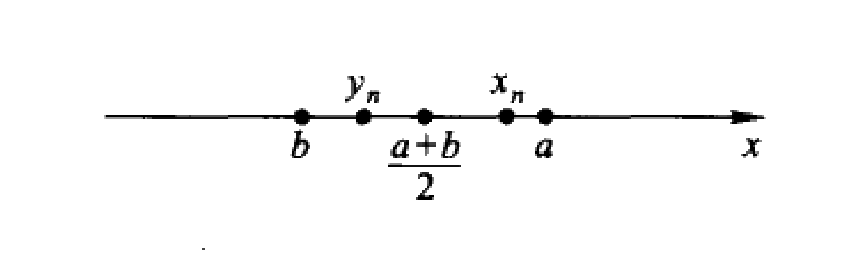
\includegraphics[width=0.55\textwidth]{work/figures/fig3-3}
\figcap\label{fig:3-3}
\end{figure}

\begin{proof}[证法 2]
令 $z_n = x_n - y_n$，则
\[
\lim_{n\to\infty}z_n = \lim_{n\to\infty}(x_n - y_n) = a - b > 0.
\]
由定理~\ref{thm:3-3}，存在 $N$，当 $n > N$ 时，有
\[
z_n = x_n - y_n > \frac{a-b}{2} > 0,
\]
即 $x_n > y_n$．这又证明了定理~\ref{thm:3-5}．
\end{proof}

值得指出的是，证法 1 用的是定理~\ref{thm:3-3} 的证明方法，证法 2 用的是定理~\ref{thm:3-3} 的结论．用定理的结论，和用定理的证明方法，是不同的两回事．对一个定理，既要学会用它的结论，也要学会用它的证明方法，这是以后学习要注意的．

\begin{theorem}[极限不等式]\label{thm:3-6}
若对任意正整数 $n$ 有 $x_n \leqslant y_n$，且 $\lim_{n \to \infty} x_n = a$，$\lim_{n \to \infty} y_n = b$，则 $a \leqslant b$．
\end{theorem}

\begin{proof}
用反证法．如果不然，设 $a > b$，则由定理~\ref{thm:3-5}，存在 $N$，当 $n > N$ 时有 $x_n > y_n$，与假设条件矛盾．故必有 $a \leqslant b$．
\end{proof}

注意到数列的前有限项并不影响数列的极限，因此定理~\ref{thm:3-6} 的条件可以减弱为``存在 $N$，当 $n > N$ 时有 $x_n \leqslant y_n$''．

如果将条件``$x_n \leqslant y_n$''改为``$x_n < y_n$''，并不能得到 $a < b$ 的结论．例如 $\frac{n-1}{n} < \frac{n+1}{n}$，但
\[
\lim_{n\to\infty}\frac{n-1}{n} = \lim_{n\to\infty}\frac{n+1}{n} = 1.
\]
可见结论也只能得到 $a \leqslant b$．定理~\ref{thm:3-6} 表明，在极限存在的前提下，可以在不等式两边取极限，但千万不要忘记``带上等号''．

用上面的方法，我们实际上已证明了极限的唯一性，即一个数列不可能有两个不同的极限值．

\begin{theorem}[唯一性]\label{thm:3-7}
若数列有极限存在，则极限是唯一的．
\end{theorem}

\begin{proof}
用反证法．如果不然，设 $\{x_n\}$ 有极限 $a$ 和 $b$，$a \neq b$，不妨设 $a < b$．对 $\varepsilon = \frac{b - a}{2} > 0$，存在 $N_1$，当 $n > N_1$ 时，有
\[
x_n < a + \varepsilon = \frac{a+b}{2},
\]
同样存在 $N_2$，当 $n > N_2$ 时，有
\[
x_n > b - \varepsilon = \frac{a+b}{2},
\]
故当 $n > \max (N_1, N_2)$ 时，有
\[
x_n < a + \varepsilon = b - \varepsilon = \frac{a+b}{2} < x_n,
\]
这是不可能的，这就证明了极限的唯一性．
\end{proof}

\begin{theorem}[夹迫性]\label{thm:3-8}
如果对任意正整数 $n$，有
\[
x_n \leqslant y_n \leqslant z_n,
\]
且 $\lim_{n\to\infty}x_n = \lim_{n\to\infty}z_n = a$，则 $\lim_{n\to\infty}y_n$ 存在且等于 $a$．
\end{theorem}

\begin{proof}
对任意给定的 $\varepsilon > 0$，由 $\lim_{n \to \infty} x_n = \lim_{n \to \infty} z_n = a$，存在 $N_1$，当 $n > N_1$ 时，有
\[
|x_n - a| < \varepsilon,\qquad \text{即}\quad a-\varepsilon < x_n < a+\varepsilon.
\]
存在 $N_2$，当 $n > N_2$ 时，有
\[
|z_n - a| < \varepsilon,\qquad \text{即}\quad a-\varepsilon < z_n < a+\varepsilon.
\]
令 $N = \max(N_1, N_2)$，则当 $n > N$ 时，有
\[
a-\varepsilon < x_n \leqslant y_n \leqslant z_n < a+\varepsilon,
\]
即
\[
|y_n - a| < \varepsilon.
\]
故 $\lim_{n\to\infty}y_n$ 存在且等于 $a$，定理证完．
\end{proof}

\begin{example}\label{ex:3-2-12}
设 $x_n = \sqrt[n]{A^n + B^n}$，其中 $A>B>0$，求证 $\lim_{n\to\infty}x_n = A$．
\end{example}

\begin{proof}
由于
\[
A = \sqrt[n]{A^n} \leqslant \sqrt[n]{A^n + B^n} \leqslant \sqrt[n]{2A^n} = \sqrt[n]{2}A,
\]
而
\[
\lim_{n\to\infty}\sqrt[n]{2}A = 1\cdot A = A,
\]
由定理~\ref{thm:3-8} 即得 $\lim_{n\to\infty}\sqrt[n]{A^n + B^n} = A$．
\end{proof}

\begin{example}\label{ex:3-2-13}
证明 $\lim_{n\to\infty}\sqrt[n]{n} = 1$．
\end{example}

\begin{proof}[证法 1]
当 $n > 1$ 时，$\sqrt[n]{n} > 1$，令 $\sqrt[n]{n} = 1 + h_n$，其中 $h_n > 0$．这时
\[
n = (1+h_n)^n = 1 + nh_n + \frac{n(n-1)}{2}h_n^2 + \cdots + h_n^n \geqslant \frac{n(n-1)}{2}h_n^2,
\]
因此 $h_n \leqslant \sqrt{\frac{2}{n-1}}$．故
\[
1 < \sqrt[n]{n} = 1 + h_n \leqslant 1 + \sqrt{\frac{2}{n-1}}.
\]
已知
\[
\lim_{n\to\infty}\left(1 + \sqrt{\frac{2}{n-1}}\right) = 1 + \lim_{n\to\infty}\sqrt{\frac{2}{n-1}} = 1,
\]
由定理~\ref{thm:3-8} 得 $\lim_{n\to\infty}\sqrt[n]{n} = 1$．
\end{proof}

\begin{proof}[证法 2]
当 $n>1$ 时，由平均值不等式得
\[
1 < \sqrt[n]{n} = \sqrt[n]{\sqrt{n}\cdot\sqrt{n}\cdot1\cdots1} \leqslant \frac{\sqrt{n} + \sqrt{n} + n - 2}{n} = \frac{2}{\sqrt{n}} + 1 - \frac{2}{n}.
\]
而
\[
\lim_{n\to\infty}\left(\frac{2}{\sqrt{n}} + 1 - \frac{2}{n}\right) = 1,
\]
由定理~\ref{thm:3-8} 得 $\lim_{n\to\infty}\sqrt[n]{n} = 1$．
\end{proof}

回忆函数单调性定义，我们说数列 $\{x_n\}$ 单调上升（下降），是指 $x_n \leqslant x_{n+1}$（$x_n \geqslant x_{n+1}$）对一切 $n$ 成立．

\begin{theorem}\label{thm:3-9}
单调上升（下降）有上（下）界的数列必有极限存在．
\end{theorem}

\begin{proof}
设数列 $\{x_n\}$ 单调上升有上界．令 $B$ 是 $\{x_n\}$ 全体上界组成的集合，即
\[
B = \{b\mid x_n \leqslant b,\,\forall n\},
\]
而
\[
A = \mathbb{R}\setminus B,
\]
则 $A \mid B$ 是实数的一个分划．事实上，由 $\{x_n\}$ 有上界，知 $B$ 不空．又 $\{x_n\}$ 单调上升，故 $x_1 - 1 \in A$，即 $A$ 不空．由 $A = \mathbb{R} \setminus B$ 知，$A,B$ 不漏．又对任给 $a \in A, b \in B$，则存在 $n_0$，使 $a < x_{n_0} \leqslant b$，即 $A,B$ 不乱．故 $A \mid B$ 是实数的一个分划．根据实数基本定理，存在 $\alpha \in \mathbb{R}$ 使得对任意 $a \in A$，任意 $b \in B$，有 $a \leqslant \alpha \leqslant b$．

下证 $\lim_{n\to\infty}x_n = \alpha$．事实上，对任给 $\varepsilon>0$，由于 $\alpha-\varepsilon \in A$，知存在 $N$，使 $\alpha-\varepsilon < x_N$，又 $\{x_n\}$ 单调上升，故当 $n>N$ 时，有 $\alpha-\varepsilon < x_N \leqslant x_n$．注意到 $\alpha+\frac{\varepsilon}{2} \in B$，便有 $x_n \leqslant \alpha+\frac{\varepsilon}{2}$，故当 $n>N$ 时有
\[
\alpha-\varepsilon < x_n \leqslant \alpha+\frac{\varepsilon}{2},
\]
于是
\[
|x_n - \alpha| < \varepsilon.
\]
这就证明了 $\lim_{n\to\infty}x_n = \alpha$．

显然，单调下降的情形同样可以用上述证明方法给出，但也可以用上述结论证明．事实上，若 $\{x_n\}$ 单调下降有下界，令 $y_n = -x_n$，则 $\{y_n\}$ 就单调上升有上界，从而有极限．设极限为 $\alpha$，则
\[
\lim_{n\to\infty}x_n = \lim_{n\to\infty}(-y_n) = -\lim_{n\to\infty}y_n = -\alpha.
\]
定理证完．
\end{proof}

定理~\ref{thm:3-9} 是只断言极限存在，而没有给出如何计算极限的第一个定理．但即使只给出极限存在，有时已能提供计算的方法．

\begin{example}\label{ex:3-2-14}
设
\[
\begin{aligned}
&x_1 = \sqrt{2},\quad x_2 = \sqrt{2+\sqrt{2}},\\
&x_{n+1} = \sqrt{2+x_n} = \sqrt{2+\sqrt{2+\cdots+\sqrt{2}}},\qquad n=2,3,\cdots,
\end{aligned}
\]
求 $\{x_n\}$ 的极限．
\end{example}

\begin{proof}[解]
显然 $\{x_n\}$ 是单调上升的，下面用数学归纳法证明 $\{x_n\}$ 有上界．显然 $x_1 = \sqrt{2} < 2$．若 $x_n \leqslant 2$，则
\[
x_{n+1} = \sqrt{2+x_n} \leqslant \sqrt{2+2} = 2.
\]
故 $\{x_n\}$ 单调上升有上界，从而必有极限．设极限为 $a$，由
\[
x_{n+1}^2 = 2 + x_n,
\]
令 $n \to \infty$，即得 $a^2 = 2 + a$．解得 $a = -1$ 或 $a = 2$．由于 $x_n \geqslant \sqrt{2}$，故必有 $a \geqslant \sqrt{2}$．舍去 $a = -1$，得 $a = 2$，即 $\lim_{n \to \infty} x_n = 2$．
\end{proof}

通常我们称定理~\ref{thm:3-9} 为单调有界原理，它的意义在于给出了数列极限存在的一个判别方法．与极限定义相比，它并不需要预先估计极限值，相反，如上例表明的，有时在用它证明了极限存在的情况下，通过极限的运算可以方便地求出极限值．但务必注意，在这里极限存在性的前提是非常重要的．考察数列 $x_n = (-1)^n$，显然 $\{x_n\}$ 的极限不存在（本节习题 10），但它满足 $x_{n+1} = -x_n$．令 $n\to\infty$ 两边取极限，便得 $a = -a$，即 $a = 0$．这显然是荒谬的结果．

最后，我们用单调有界原理证明一个重要数列极限的存在性．

\begin{example}\label{ex:3-2-15}
证明数列 $\left\{\left(1+\frac{1}{n}\right)^n\right\}$ 的极限存在．
\end{example}

\begin{proof}
先证 $\left\{\left(1+\frac{1}{n}\right)^n\right\}$ 是单调上升的，即证
\[
\left(1+\frac{1}{n}\right)^n \leqslant \left(1+\frac{1}{n+1}\right)^{n+1},
\]
或
\[
\sqrt[n+1]{\left(1+\frac{1}{n}\right)^n} \leqslant 1 + \frac{1}{n+1}.
\]
由平均值不等式即得
\[
\sqrt[n+1]{\left(1+\frac{1}{n}\right)^n\cdot 1} \leqslant \frac{n\left(1+\frac{1}{n}\right) + 1}{n+1} = 1 + \frac{1}{n+1}.
\]
再证 $\left\{\left(1+\frac{1}{n}\right)^n\right\}$ 有上界．我们试图证明 $\left(1+\frac{1}{n}\right)^n < 4$．即要证
\[
\sqrt[n]{\frac{1}{4}} < \frac{n}{n+1}.
\]
此式当 $n=1$ 时显然成立，当 $n>1$ 时，由平均值不等式即得
\[
\sqrt[n]{\frac{1}{4}} = \sqrt[n]{\frac{1}{2}\cdot\frac{1}{2}\cdot1\cdots1} \leqslant \frac{\frac{1}{2} + \frac{1}{2} + (n-2)}{n} = 1 - \frac{1}{n} < 1 - \frac{1}{n+1} = \frac{n}{n+1}.
\]
故由单调有界原理知 $\lim_{n\to\infty}\left(1+\frac{1}{n}\right)^n$ 存在．
\end{proof}

通常我们记这个极限为 $\mathrm{e}$，它是一个无理数，用前几位小数表示即为
\[
\lim_{n\to\infty}\left(1+\frac{1}{n}\right)^n = \mathrm{e} = 2.718\,281\,8\cdots.
\]
称以 $\mathrm{e}$ 为底的对数为自然对数，记为 $\log_{\mathrm{e}}x = \ln x$．为什么称这是``自然对数''，读者学到后面便会明白．

\subsection*{3. 无穷大量}

在发散的数列中有一种特殊的数列，就是当 $n$ 无限增大时，$|x_n|$ 也无限增大，例如 $\{n^2\}$ 和 $\{(-2)^n\}$．我们称这种数列为无穷大量．仿照数列极限的 $\varepsilon-N$ 语言，我们给出无穷大量的严格定义．

\begin{definition}\label{def:3-4}
设 $\{x_n\}$ 是一数列．若对于任意给定的 $G > 0$，存在正整数 $N$，当 $n > N$ 时，有 $|x_n| > G$，则称 $\{x_n\}$ 是无穷大量，记为
\[
\lim_{n\to\infty}x_n = \infty,\qquad \text{或}\qquad x_n \to \infty\quad(n\to\infty).
\]
\end{definition}

值得指出的是，尽管这里仍沿用记号 $\lim_{n\to\infty}x_n = \infty$，同样我们也常沿用说法``$\{x_n\}$ 的极限为 $\infty$''，但这仅仅是为了书写和语言的方便，并不意味着 $\{x_n\}$ 收敛和 $\{x_n\}$ 的极限存在，我们说 $\{x_n\}$ 的极限存在，指的是极限值是一个数．

从几何上看，无穷大量是指任意给定区间 $[-G,G]$，必然从某项 $x_{N+1}$ 起，后面的所有项都落在区间 $[-G,G]$ 之外．换句话说，数列 $\{x_n\}$ 至多有 $N$ 项 $x_1, x_2, \cdots, x_N$ 落在区间 $[-G,G]$ 之中．

\begin{example}\label{ex:3-2-16}
证明 $\{x_n\} = \{(-2)^n\}$ 是无穷大量．
\end{example}

\begin{proof}
对任意给定的 $G>0$，不妨设 $G>2$，要使
\[
|x_n| = |(-2)^n| = 2^n > G,
\]
即
\[
n\ln2 > \ln G,
\]
只要 $n > \frac{\ln G}{\ln 2}$．令 $N = \left[\frac{\ln G}{\ln 2}\right]$，则当 $n > N$ 时，有 $|(-2)^n| > G$，即 $\{x_n\}$ 是无穷大量．
\end{proof}

类似地我们可以给出 $\lim_{n\to\infty}x_n = +\infty$ 和 $\lim_{n\to\infty}x_n = -\infty$ 的定义，分别称为 $\{x_n\}$ 是正无穷大量和 $\{x_n\}$ 是负无穷大量．例如，$\lim_{n\to\infty}x_n = +\infty$ 定义为：对任意给定的 $G>0$，存在 $N$，当 $n>N$ 时，有 $x_n > G$．

显然，若 $\{x_n\}$ 是正（负）无穷大量，则必是无穷大量；若 $\{x_n\}$ 是无穷大量，则 $\{|x_n|\}$ 是正无穷大量．

\begin{example}\label{ex:3-2-17}
证明 $\lim_{n\to\infty}n^2 = +\infty$．
\end{example}

\begin{proof}
对任意给定的 $G > 0$，不妨设 $G > 1$，要使 $n^2 > G$，只要 $n > \sqrt{G}$．取 $N = [\sqrt{G}]$，则当 $n > N$ 时，有 $n^2 > G$，故 $\lim_{n\to\infty} n^2 = +\infty$．
\end{proof}

下面我们列出无穷大量的运算法则和性质：
\begin{enumerate}
\item 无穷大量与无穷小量的关系：$\{x_n\}$ 是无穷大量当且仅当 $\left\{\frac{1}{x_n}\right\}$ 是无穷小量．
\item 若 $\{x_n\},\{y_n\}$ 是正（负）无穷大量，则 $\{x_n + y_n\}$ 是正（负）无穷大量．
\item 若 $\{x_n\}$ 是无穷大量，$\{y_n\}$ 是有界量，则 $\{x_n \pm y_n\}$ 是无穷大量．
\item 若 $\{x_n\}$ 是无穷大量，$\{y_n\}$ 满足：对给定的 $\delta > 0$，存在 $N$，当 $n > N$ 时，有 $|y_n| > \delta$，则 $\{x_n y_n\}$ 是无穷大量．
\end{enumerate}

请读者完成上述运算法则和性质的证明．

\begin{example}\label{ex:3-2-18}
若 $\lim_{n\to\infty}x_n = a \neq 0$，$\lim_{n\to\infty}y_n = \infty$，则 $\lim_{n\to\infty}x_n y_n = \infty$．
\end{example}

\begin{proof}
由 $\lim_{n\to\infty}x_n = a \neq 0$，则存在 $N_1$，当 $n>N_1$ 时，有
\[
|x_n| > \frac{|a|}{2} > 0.
\]
由 $\lim_{n\to\infty}y_n = \infty$，则对任意给定的 $G>0$，存在 $N_2$，当 $n>N_2$ 时，有
\[
|y_n| > \frac{2}{|a|}G.
\]
令 $N = \max(N_1, N_2)$，则当 $n > N$ 时，有
\[
|x_n y_n| > \frac{|a|}{2}|y_n| > G,
\]
所以 $\lim_{n\to\infty}x_n y_n = \infty$．
\end{proof}

\begin{example}\label{ex:3-2-19}
证明 $\lim_{n\to\infty}\frac{2n^2+n+1}{3n-4} = \infty$．
\end{example}

\begin{proof}[解]
由于 $\lim_{n\to\infty}\frac{3n-4}{2n^2+n+1} = 0$，利用无穷大量和无穷小量的关系即得证．
\end{proof}

综合上例和例~\ref{ex:3-2-11}，当 $a_0 \neq 0$，$b_0 \neq 0$ 时有
\[
\lim_{n\to\infty}\frac{a_0 n^k + a_1 n^{k-1} + \cdots + a_k}{b_0 n^l + b_1 n^{l-1} + \cdots + b_l} = \begin{cases}
\frac{a_0}{b_0}, & k = l,\\
0, & k < l,\\
\infty, & k > l.
\end{cases}
\]

\begin{xiti}
\item 用定义证明下列数列的极限为零：
  \begin{ziti}
  \item $\lim_{n \to \infty} \frac{n + 1}{n^2 + 1} = 0$；
  \item $\lim_{n \to \infty} \frac{\sin n}{n} = 0$；
  \item $\lim_{n \to \infty} \frac{1}{n!} = 0$；
  \item $\lim_{n \to \infty} \frac{n + (-1)^n}{n^2 - 1} = 0$；
  \item $\lim_{n \to \infty} (\sqrt{n + 1} - \sqrt{n}) = 0$；
  \item $\lim_{n \to \infty} \frac{10^n}{n!} = 0$；
  \item $\lim_{n \to \infty} \frac{n}{a^n} = 0\quad (a > 1)$；
  \item $\lim_{n \to \infty} \frac{n!}{n^n} = 0$；
  \item $\lim_{n \to \infty} \frac{1 + 2 + 3 + \cdots + n}{n^3} = 0$；
  \item $\lim_{n \to \infty} (\frac{1}{n} + a^{-n}) = 0\quad (a > 1)$．
  \end{ziti}
\item 用定义证明：
  \begin{ziti}
  \item $\lim_{n \to \infty} \frac{3n^2 + n}{2n^2 - 1} = \frac{3}{2}$；
  \item $\lim_{n \to \infty} \frac{\sqrt{n^2 + n}}{n} = 1$；
  \item $\lim_{n\to\infty}x_n = 1$，其中 $x_n = \begin{cases} \frac{n-1}{n}, & n\text{ 为偶数},\\ \frac{n+1}{n}, & n\text{ 为奇数}; \end{cases}$
  \item $\lim_{n \to \infty} x_n = 3$，其中 $x_n = \begin{cases} 3, & n = 3k,\\ \frac{3n+1}{n}, & n = 3k+1,\\ 2 + \frac{1+n}{3-\sqrt{n}+n}, & n = 3k+2 \end{cases}\quad (k=1,2,\cdots)$．
  \end{ziti}
\item 用定义证明：
  \begin{ziti}
  \item 若 $\lim_{n\to\infty}a_n = a$，则对任一正整数 $k$，有 $\lim_{n\to\infty}a_{n+k} = a$；
  \item 若 $\lim_{n\to\infty}a_n = a$，则 $\lim_{n\to\infty}|a_n| = |a|$．反之是否成立？
  \item 若 $\lim_{n\to\infty}a_n = a$，且 $a>b$，则存在 $N$，当 $n>N$ 时，有 $a_n > b$；
  \item 若 $\lim_{n\to\infty}a_n = a$，且 $a_n > 0$，则 $\lim_{n\to\infty}\sqrt{a_n} = \sqrt{a}$．
  \end{ziti}
\item 极限的定义改成下面形式是否可以？（其中``$\exists$''是逻辑符号，表示``存在''）
  \begin{ziti}
  \item $\forall \varepsilon > 0, \exists N > 0$，当 $n \geqslant N$ 时，有 $|x_n - a| < \varepsilon$；
  \item $\forall \varepsilon > 0, \exists N > 0$，当 $n > N$ 时，有 $|x_n - a| \leqslant \varepsilon$；
  \item $\forall \varepsilon > 0, \exists N > 0$，当 $n > N$ 时，有 $|x_n - a| < M\varepsilon$（$M$ 为常数）．
  \end{ziti}
\item 若 $\{x_n y_n\}$ 收敛，能否断定 $\{x_n\}$、$\{y_n\}$ 也收敛？
\item 设 $x_n \leqslant a \leqslant y_n$ ($n = 1, 2, \cdots$)，且 $\lim_{n \to \infty} (y_n - x_n) = 0$，求证：
\[
\lim_{n\to\infty}x_n = a,\qquad \lim_{n\to\infty}y_n = a.
\]
\item 利用极限的四则运算法则求极限：
  \begin{ziti}
  \item $\lim_{n \to \infty} \frac{3n^3 + 2n^2 - n + 1}{2n^3 - 3n^2 + 2}$；
  \item $\lim_{n\to\infty}\frac{(-2)^n + 3^n}{(-2)^{n+1} + 3^{n+1}}$；
  \item $\lim_{n \to \infty} \frac{1 + \frac{1}{2} + \cdots + \frac{1}{2^n}}{1 + \frac{1}{4} + \cdots + \frac{1}{4^n}}$；
  \item $\lim_{n \to \infty} (\sqrt[n]{1} + \sqrt[n]{2} + \cdots + \sqrt[n]{10})$．
  \end{ziti}
\item 求下列极限：
  \begin{ziti}
  \item $\lim_{n \to \infty} \left[\frac{1}{1 \cdot 2} + \frac{1}{2 \cdot 3} + \cdots + \frac{1}{n(n+1)}\right]$；
  \item $\lim_{n\to\infty}\left[\frac{1}{n^2} + \frac{1}{(n+1)^2} + \cdots + \frac{1}{(2n)^2}\right]$；
  \item $\lim_{n \to \infty} \left(\frac{1}{\sqrt{n^2 + 1}} + \frac{1}{\sqrt{n^2 + 2}} + \cdots + \frac{1}{\sqrt{n^2 + n}}\right)$；
  \item $\lim_{n\to\infty}\left(\frac{1}{2} + \frac{3}{2^2} + \cdots + \frac{2n-1}{2^n}\right)$；
  \item $\lim_{n \to \infty} \left(1 - \frac{1}{\sqrt[n]{2}}\right) \cos n$；
  \item $\lim_{n \to \infty} \sqrt{1 - \frac{1}{n}}$；
  \item $\lim_{n \to \infty} (\sqrt{2} \sqrt[4]{2} \sqrt[8]{2} \cdots \sqrt[2^n]{2})$；
  \item $\lim_{n \to \infty} \left[(n + 1)^\alpha - n^\alpha\right],\quad 0 < \alpha < 1$；
  \item $\lim_{n \to \infty} \frac{1}{2} \cdot \frac{3}{4} \cdots \frac{2n-1}{2n}$；
  \item $\lim_{n \to \infty} \sqrt[n]{\frac{1 \cdot 3 \cdot 5 \cdots (2n-1)}{2 \cdot 4 \cdot 6 \cdots (2n)}}$；
  \item $\lim_{n \to \infty} \frac{1}{\sqrt[n]{n!}}$；
  \item $\lim_{n \to \infty} \sqrt[n]{n \ln n}$．
  \end{ziti}
\item 证明：若 $\{a_n\},\{b_n\}$ 中一个是收敛数列，另一个是发散数列，则 $\{a_n \pm b_n\}$ 是发散数列；又问 $\{a_n b_n\}$ 和 $\left\{\frac{a_n}{b_n}\right\}$ ($b_n \neq 0$) 是否也是发散数列？为什么？
\item 设 $x_n = (-1)^n$，证明 $\{x_n\}$ 发散．
\item 若 $a_1, a_2, \cdots, a_m$ 为 $m$ 个正数，证明：
\[
\lim_{n\to\infty}\sqrt[n]{a_1^n + a_2^n + \cdots + a_m^n} = \max(a_1, a_2, \cdots, a_m).
\]
\item 设 $\lim_{n\to\infty}a_n = a$，证明：
  \begin{ziti}
  \item $\lim_{n \to \infty} \frac{[n a_n]}{n} = a$；
  \item 若 $a > 0$，$a_n > 0$，则 $\lim_{n \to \infty} \sqrt[n]{a_n} = 1$．
  \end{ziti}
\item 利用单调有界原理，证明 $\lim_{n\to\infty}x_n$ 存在，并求出它：
  \begin{ziti}
  \item $x_1 = \sqrt{2}$，$x_n = \sqrt{2 x_{n-1}}$，$n=2,3,\cdots$；
  \item $x_1 = \sqrt{c} > 0$，$x_n = \sqrt{c + x_{n-1}}$，$n=2,3,\cdots$；
  \item $x_n = \frac{c^n}{n!}\quad (c > 0)$；
  \item $x_0 = 1$，$x_n = 1 + \frac{x_{n-1}}{1 + x_{n-1}}$，$n=1,2,\cdots$．
  \end{ziti}
\item 若 $x_1 = a > 0$，$y_1 = b > 0$ ($a < b$)，
\[
x_{n+1} = \sqrt{x_n y_n},\qquad y_{n+1} = \frac{x_n + y_n}{2},
\]
证明：$\lim_{n\to\infty}x_n = \lim_{n\to\infty}y_n$．
\item 证明：若 $a_n > 0$，且 $\lim_{n\to\infty}\frac{a_n}{a_{n+1}} = l > 1$，则 $\lim_{n\to\infty}a_n = 0$．
\item 设 $\lim_{n\to\infty}a_n = a$，证明：
  \begin{ziti}
  \item $\lim_{n\to\infty}\frac{a_1 + a_2 + \cdots + a_n}{n} = a$；（又问，它的逆命题成立否？）
  \item 若 $a_n > 0$，则 $\lim_{n \to \infty} \sqrt[n]{a_1 a_2 \cdots a_n} = a$．
  \end{ziti}
\item 应用上题的结果证明下列各题：
  \begin{ziti}
  \item $\lim_{n \to \infty} \frac{1 + \frac{1}{2} + \frac{1}{3} + \cdots + \frac{1}{n}}{n} = 0$；
  \item $\lim_{n \to \infty} \sqrt[n]{a} = 1\quad (a > 0)$；
  \item $\lim_{n \to \infty} \sqrt[n]{n} = 1$；
  \item $\lim_{n \to \infty} \frac{1}{\sqrt[n]{n!}} = 0$；
  \item $\lim_{n \to \infty} \frac{1 + \sqrt{2} + \sqrt[3]{3} + \cdots + \sqrt[n]{n}}{n} = 1$；
  \item 若 $\lim_{n\to\infty}\frac{b_{n+1}}{b_n} = a$ ($b_n > 0$)，则 $\lim_{n\to\infty}\sqrt[n]{b_n} = a$．
  \end{ziti}
\item 用定义证明下列数列为无穷大量：
  \begin{ziti}
  \item $\{\sqrt{n}\}$；
  \item $\{n!\}$；
  \item $\{\ln n\}$；
  \item $1 + \frac{1}{2} + \frac{1}{3} + \cdots + \frac{1}{n}$．
  \end{ziti}
\item 证明：若 $\{x_n\}$ 为无穷大量，$\{y_n\}$ 为有界变量，则 $\{x_n \pm y_n\}$ 为无穷大量．
\item 讨论题：
  \begin{ziti}
  \item 两个无穷大量的和的极限如何？试讨论各种可能情形；
  \item 讨论无穷大量和无穷小量的和、差、商的极限的情形；
  \item 讨论无穷大量和无穷小量的乘积可能发生的各种情形．
  \end{ziti}
\item 利用 $\lim_{n\to\infty}\left(1+\frac{1}{n}\right)^n = \mathrm{e}$，求下列极限：
  \begin{ziti}
  \item $\lim_{n \to \infty} \left(1 - \frac{1}{n}\right)^n$；
  \item $\lim_{n \to \infty} \left(1 + \frac{1}{n + 1}\right)^n$．
  \end{ziti}
\end{xiti}

\section{函数的极限}\label{sec:3.3}

我们现在来讨论函数的极限．注意，典型的函数极限模型来自对自由落体运动，由平均速度
\[
\frac{\frac{1}{2}g(t+h)^2 - \frac{1}{2}gt^2}{h}
\]
求瞬时速度．也就是说要考察上述 $h$ 的函数（注意，$t$ 是固定的），当 $h$ 无限变小时，它的变化趋势，即看它是否无限接近于一个数．

首先看到，这个函数在 $h=0$ 是没有定义的，但至少在包含 $0$ 的一个开区间（$0$ 这点除外）有定义．$h$ 不等于 $0$ 时，有
\[
\frac{\frac{1}{2}g(t+h)^2 - \frac{1}{2}gt^2}{h} = gt + \frac{1}{2}gh.
\]
当 $|h|$ 很小时，左边的函数值与 $gt$ 的差也很小，而且当 $h$ 无限接近于 $0$（而不等于 $0$）时，左边的函数也就无限接近于 $gt$．

重复数列极限时的讨论，把``接近''、``无限''等语言精确化，便得到一般的函数极限概念的定义．

\begin{definition}\label{def:3-5}
设 $f(x)$ 在 $x_0$ 点附近（$x_0$ 除外）有定义，$A$ 为一常数．如果任给 $\varepsilon > 0$，存在 $\delta > 0$，使得当 $0 < |x - x_0| < \delta$ 时，有
\[
|f(x) - A| < \varepsilon,
\]
则称 $A$ 是函数 $f(x)$ 当 $x$ 趋于 $x_0$ 时的极限，记为
\[
\lim_{x \to x_0} f(x) = A \quad \text{或} \quad f(x) \to A \quad (x \to x_0).
\]
\end{definition}

也可以说成：$f(x)$ 当 $x \to x_0$ 时有极限 $A$．

在定义中用到的符号 $\delta$，在概念上对应于数列极限中的 $N$．在数列极限中，$n \to \infty$ 是用 $n > N$ 来刻画；而在函数极限中，$x \to x_0$ 则是用 $0 < |x - x_0| < \delta$ 来刻画．$\delta$ 越小，说明 $x$ 越接近 $x_0$．

在定义中，需要注意的是，函数在 $x_0$ 这点是否有定义，对函数在 $x_0$ 点有无极限，是毫无关系的．定义中的条件 $0 < |x - x_0| < \delta$，意味着 $x \neq x_0$，所以即使函数在 $x_0$ 这点没有定义，或者虽然有定义但函数值 $f(x_0)$ 与极限值 $A$ 并不相等，这并不妨碍极限的存在．

\begin{figure}[htbp]
\centering
\includegraphics[width=0.65\textwidth]{fig3-4.png}
\figcap
\label{fig:3-4}
\end{figure}

注意到不等式 $|f(x) - A| < \varepsilon$ 等价于 $A - \varepsilon < f(x) < A + \varepsilon$，函数 $f(x)$ 当 $x \to x_0$ 时的极限为 $A$ 的几何解释便是（图~\ref{fig:3-4}）：任给 $\varepsilon > 0$，作直线 $y = A - \varepsilon$ 和 $y = A + \varepsilon$．这时必存在 $\delta > 0$，使得在两垂线 $x = x_0 - \delta$ 与 $x = x_0 + \delta$ 之间（垂线 $x = x_0$ 除外）的曲线 $y = f(x)$，全部落在两平行直线 $y = A - \varepsilon$ 与 $y = A + \varepsilon$ 所夹的带形区域内．

\begin{example}\label{ex:3-3-1}
证明
\[
\lim_{h \to 0} \frac{\frac{1}{2}g(t+h)^2 - \frac{1}{2}gt^2}{h} = gt.
\]
\end{example}

\begin{proof}
任给 $\varepsilon > 0$．由
\[
\left|\frac{\frac{1}{2}g(t+h)^2 - \frac{1}{2}gt^2}{h} - gt\right| = \left|gt + \frac{1}{2}gh - gt\right| = \frac{g}{2}|h|,
\]
要使
\[
\left|\frac{\frac{1}{2}g(t+h)^2 - \frac{1}{2}gt^2}{h} - gt\right| < \varepsilon,
\]
只要取 $\delta = \frac{2\varepsilon}{g}$，则当 $0 < |h| < \delta$ 时，便有
\[
\left|\frac{\frac{1}{2}g(t+h)^2 - \frac{1}{2}gt^2}{h} - gt\right| = \frac{g}{2}|h| < \frac{g}{2} \cdot \frac{2\varepsilon}{g} = \varepsilon.
\]
这就证明了所要证明的结论．
\end{proof}

从这便看到了极限概念的妙处．牛顿当时的瞬 $h$ 是 0 还是非 0 的矛盾就解决了．这里的 $h$ 先作为一个变动的量，从两边（一个非 0 的对称区间）无限接近于 $0$（但不等于 $0$），在这个过程中看平均速度的变化趋势，即极限．

\begin{example}\label{ex:3-3-2}
证明 $\lim_{x \to a} \sqrt{x} = \sqrt{a}$，这里 $a > 0$．
\end{example}

\begin{proof}
任给 $\varepsilon > 0$．当 $x > 0$ 时，
\[
|\sqrt{x} - \sqrt{a}| = \frac{|x - a|}{\sqrt{x} + \sqrt{a}} < \frac{|x - a|}{\sqrt{a}}.
\]
因此，只要取 $\delta = \sqrt{a}\varepsilon$，则当 $0 < |x - a| < \delta$ 时，便有
\[
|\sqrt{x} - \sqrt{a}| < \frac{|x - a|}{\sqrt{a}} < \frac{\delta}{\sqrt{a}} = \varepsilon.
\]
即 $\lim_{x \to a} \sqrt{x} = \sqrt{a}$．
\end{proof}

\begin{example}\label{ex:3-3-3}
证明 $\lim_{x \to 1} \frac{x^3 - 1}{x - 1} = 3$．
\end{example}

\begin{proof}
任给 $\varepsilon > 0$．当 $x \neq 1$ 时，
\[
\left|\frac{x^3 - 1}{x - 1} - 3\right| = |x^2 + x + 1 - 3| = |x^2 + x - 2| = |x - 1||x + 2|.
\]
限制 $|x - 1| < 1$，即 $0 < x < 2$．此时
\[
|x + 2| < 4.
\]
从而
\[
\left|\frac{x^3 - 1}{x - 1} - 3\right| < 4|x - 1|.
\]
因此取 $\delta = \min\left\{1, \frac{\varepsilon}{4}\right\}$，则当 $0 < |x - 1| < \delta$ 时，有
\[
\left|\frac{x^3 - 1}{x - 1} - 3\right| < 4|x - 1| < 4 \cdot \frac{\varepsilon}{4} = \varepsilon.
\]
即 $\lim_{x \to 1} \frac{x^3 - 1}{x - 1} = 3$．
\end{proof}

这里所用的方法仍然是``适当放大法''．因为 $x$ 是连续变动的，所以一开始就要对 $x$ 的变化范围作一定的限制，以便以后能适当放大 $|f(x) - A|$，从而能较方便地找到一个 $\delta$．

对于函数的极限，同样也有对应于数列极限的一系列的性质，其证明也是类似的，关键是要找到两者的联系．例如，在数列极限中是``存在 $N$，只要 $n > N$''，而在函数极限中则为``存在 $\delta > 0$，只要 $0 < |x - x_0| < \delta$''．自然也有各地方，函数极限与数列极限是很不相同的，读者应特别注意．

\begin{theorem}[四则运算]\label{thm:3-1-prime}
设 $\lim_{x \to x_0} f(x) = A$，$\lim_{x \to x_0} g(x) = B$，则
\begin{enumerate}[label=(\roman*)]
\item $\lim_{x \to x_0} [f(x) \pm g(x)] = A \pm B$；
\item $\lim_{x \to x_0} [f(x)g(x)] = AB$；
\item 当 $B \neq 0$ 时，$\lim_{x \to x_0} \frac{f(x)}{g(x)} = \frac{A}{B}$．
\end{enumerate}
\end{theorem}

\begin{theorem}[局部有界性]\label{thm:3-2-prime}
设 $\lim_{x \to x_0} f(x) = A$，则存在常数 $M > 0$ 与 $\delta > 0$，使得当 $0 < |x - x_0| < \delta$ 时，有
\[
|f(x)| \leqslant M.
\]
\end{theorem}

\begin{theorem}[局部保号性]\label{thm:3-3-prime}
设 $\lim_{x \to x_0} f(x) = A$．如果 $A > 0$（或 $A < 0$），则存在 $\delta > 0$，使得当 $0 < |x - x_0| < \delta$ 时，有
\[
f(x) > 0 \quad (\text{或 } f(x) < 0).
\]
特别地，当 $A > 0$ 时，存在 $\delta > 0$，使得当 $0 < |x - x_0| < \delta$ 时，有
\[
f(x) > \frac{A}{2}.
\]
\end{theorem}

\begin{proof}
由 $\lim_{x \to x_0} f(x) = A$，对 $\varepsilon = \frac{A}{2} > 0$，存在 $\delta > 0$，使得当 $0 < |x - x_0| < \delta$ 时，有
\[
|f(x) - A| < \frac{A}{2},
\]
即
\[
A - \frac{A}{2} < f(x) < A + \frac{A}{2}.
\]
从而
\[
f(x) > A - \frac{A}{2} = \frac{A}{2} > 0.
\]
定理~\ref{thm:3-3-prime} 证毕．
\end{proof}

\begin{theorem}[无穷小与局部有界函数之积]\label{thm:3-4-prime}
若 $\lim_{x \to x_0} \alpha(x) = 0$，且存在 $M > 0$ 及 $\delta_1 > 0$，使得当 $0 < |x - x_0| < \delta_1$ 时，有 $|g(x)| \leqslant M$，则
\[
\lim_{x \to x_0} \alpha(x)g(x) = 0.
\]
\end{theorem}

下面我们来证明定理~\ref{thm:3-1-prime}．

\begin{proof}[定理~\ref{thm:3-1-prime}的证明]
(i) 的证明是简单的，留给读者，这里只证 (ii) 与 (iii)．

(ii) 因为
\[
|f(x)g(x) - AB| = |f(x)g(x) - Ag(x) + Ag(x) - AB| \leqslant |g(x)||f(x) - A| + |A||g(x) - B|.
\]
由 $\lim_{x \to x_0} g(x) = B$，由局部有界性（定理~\ref{thm:3-2-prime}），存在 $\delta_1 > 0$ 及 $M > 0$，使得当 $0 < |x - x_0| < \delta_1$ 时，有 $|g(x)| \leqslant M$．

任给 $\varepsilon > 0$，由 $\lim_{x \to x_0} f(x) = A$，$\lim_{x \to x_0} g(x) = B$，存在 $\delta_2 > 0$，使得当 $0 < |x - x_0| < \delta_2$ 时，有
\[
|f(x) - A| < \frac{\varepsilon}{2M} \quad \text{与} \quad |g(x) - B| < \frac{\varepsilon}{2(|A| + 1)}.
\]
取 $\delta = \min\{\delta_1, \delta_2\}$，则当 $0 < |x - x_0| < \delta$ 时，
\[
|f(x)g(x) - AB| < M \cdot \frac{\varepsilon}{2M} + |A| \cdot \frac{\varepsilon}{2(|A| + 1)} < \frac{\varepsilon}{2} + \frac{\varepsilon}{2} = \varepsilon.
\]
这就证明了 $\lim_{x \to x_0} [f(x)g(x)] = AB$．

(iii) 设 $B \neq 0$．由于
\[
\left|\frac{f(x)}{g(x)} - \frac{A}{B}\right| = \frac{|B f(x) - A g(x)|}{|B||g(x)|} = \frac{|B(f(x) - A) - A(g(x) - B)|}{|B||g(x)|} \leqslant \frac{|f(x) - A|}{|g(x)|} + \frac{|A||g(x) - B|}{|B||g(x)|}.
\]
由局部保号性（定理~\ref{thm:3-3-prime}），存在 $\delta_1 > 0$，当 $0 < |x - x_0| < \delta_1$ 时，有 $|g(x)| > \frac{|B|}{2}$，从而 $\frac{1}{|g(x)|} < \frac{2}{|B|}$．

因此，当 $0 < |x - x_0| < \delta_1$ 时，有
\[
\left|\frac{f(x)}{g(x)} - \frac{A}{B}\right| < \frac{2}{|B|}|f(x) - A| + \frac{2|A|}{|B|^2}|g(x) - B|.
\]
任给 $\varepsilon > 0$，由 $\lim_{x \to x_0} f(x) = A$ 及 $\lim_{x \to x_0} g(x) = B$，存在 $\delta_2 > 0$，当 $0 < |x - x_0| < \delta_2$ 时，有
\[
|f(x) - A| < \frac{|B|}{4}\varepsilon,
\]
且存在 $\delta_3 > 0$，当 $0 < |x - x_0| < \delta_3$ 时，有
\[
|g(x) - B| < \frac{|B|^2}{4(|A| + 1)}\varepsilon.
\]
取 $\delta = \min\{\delta_1, \delta_2, \delta_3\}$，则当 $0 < |x - x_0| < \delta$ 时，便有
\[
\left|\frac{f(x)}{g(x)} - \frac{A}{B}\right| < \frac{2}{|B|} \cdot \frac{|B|}{4}\varepsilon + \frac{2|A|}{|B|^2} \cdot \frac{|B|^2}{4(|A| + 1)}\varepsilon < \frac{\varepsilon}{2} + \frac{\varepsilon}{2} = \varepsilon.
\]
故 $\lim_{x \to x_0} \frac{f(x)}{g(x)} = \frac{A}{B}$．定理~\ref{thm:3-1-prime} 证毕．
\end{proof}

对应于数列极限的性质，我们还有：

\begin{theorem}[局部保序性]\label{thm:3-5-prime}
设 $\lim_{x \to x_0} f(x) = A$，$\lim_{x \to x_0} g(x) = B$．若 $A < B$，则存在 $\delta > 0$，使得当 $0 < |x - x_0| < \delta$ 时，有
\[
f(x) < g(x).
\]
\end{theorem}

\begin{theorem}[极限不等式]\label{thm:3-6-prime}
设 $\lim_{x \to x_0} f(x) = A$，$\lim_{x \to x_0} g(x) = B$．若存在 $\delta_0 > 0$，使得当 $0 < |x - x_0| < \delta_0$ 时，有 $f(x) \leqslant g(x)$，则
\[
A \leqslant B.
\]
\end{theorem}

\begin{theorem}[极限唯一性]\label{thm:3-7-prime}
如果极限 $\lim_{x \to x_0} f(x)$ 存在，则极限是唯一的．
\end{theorem}

\begin{theorem}[夹迫性]\label{thm:3-8-prime}
若存在 $\delta > 0$，使得当 $0 < |x - x_0| < \delta$ 时，有
\[
g(x) \leqslant f(x) \leqslant h(x),
\]
且 $\lim_{x \to x_0} g(x) = \lim_{x \to x_0} h(x) = A$，则
\[
\lim_{x \to x_0} f(x) = A.
\]
\end{theorem}

这些定理的证明完全与数列极限的情形类似，请读者自己写出．

由定理~\ref{thm:3-8-prime}，容易得出以下两个推论：

\begin{corollary}\label{cor:3-3-prime}
设 $\lim_{x \to x_0} g(x) = 0$．如果存在 $\delta > 0$，使得当 $0 < |x - x_0| < \delta$ 时，有
\[
|f(x)| \leqslant g(x),
\]
则 $\lim_{x \to x_0} f(x) = 0$．
\end{corollary}

\begin{corollary}\label{cor:3-4}
设 $\lim_{x \to x_0} g(x) = 0$．如果存在 $\delta > 0$ 及常数 $A$，使得当 $0 < |x - x_0| < \delta$ 时，有
\[
|f(x) - A| \leqslant g(x),
\]
则 $\lim_{x \to x_0} f(x) = A$．
\end{corollary}

由数列极限的定义，读者也许已注意到对应于数列的极限过程 $n \to \infty$，函数的极限过程可以通过自变量取值于数列 $x_n \to x_0$ 来实现．即不仅可以把一个函数的极限过程看作连续过程，也可以看作某种离散过程的某种结合．这种看法可以由海涅（Heine）提出的下面的定理所体现．

\begin{theorem}[海涅定理，归结原则]\label{thm:3-10}
$\lim_{x \to x_0} f(x) = A$ 的充要条件是：对任何满足 $x_n \neq x_0$ 且 $\lim_{n \to \infty} x_n = x_0$ 的数列 $\{x_n\}$，都有
\[
\lim_{n \to \infty} f(x_n) = A.
\]
\end{theorem}

\begin{proof}
必要性．已知 $\lim_{x \to x_0} f(x) = A$．任给 $\varepsilon > 0$，存在 $\delta > 0$，使得当 $0 < |x - x_0| < \delta$ 时，有
\[
|f(x) - A| < \varepsilon.
\]
对于任何满足 $x_n \neq x_0$ 且 $\lim_{n \to \infty} x_n = x_0$ 的数列 $\{x_n\}$，对上述的 $\delta > 0$，存在自然数 $N$，使得当 $n > N$ 时，有
\[
0 < |x_n - x_0| < \delta.
\]
从而当 $n > N$ 时，有
\[
|f(x_n) - A| < \varepsilon.
\]
这就证明了 $\lim_{n \to \infty} f(x_n) = A$．

充分性．用反证法．如果 $\lim_{x \to x_0} f(x) = A$ 不成立，即存在某个 $\varepsilon_0 > 0$，对任何 $\delta > 0$，存在 $x_\delta$，满足 $0 < |x_\delta - x_0| < \delta$，但
\[
|f(x_\delta) - A| \geqslant \varepsilon_0.
\]
特别取 $\delta = \frac{1}{n}$ ($n = 1, 2, \cdots$)，则对每个 $n$，相应地存在 $x_n$，使得
\[
0 < |x_n - x_0| < \frac{1}{n} \quad \text{但} \quad |f(x_n) - A| \geqslant \varepsilon_0.
\]
显然，此数列满足 $x_n \neq x_0$ 且 $\lim_{n \to \infty} x_n = x_0$．但由于对一切 $n$，都有 $|f(x_n) - A| \geqslant \varepsilon_0$，所以 $\{f(x_n)\}$ 不可能以 $A$ 为极限．这与充分性的假设矛盾！因此必有 $\lim_{x \to x_0} f(x) = A$．
\end{proof}

既然函数极限可以通过数列极限来刻画，那么我们就可以利用这种刻画把数列极限的一些性质移植到函数极限，例如定理~\ref{thm:3-6-prime}、定理~\ref{thm:3-8-prime}等的证明，也可以用定理~\ref{thm:3-10}来完成．

定理~\ref{thm:3-10}不仅可以用来证明某些函数极限存在，更重要的在于证明某些函数极限不存在．

\begin{example}\label{ex:3-3-4}
证明 $\lim_{x \to 0} \sin\frac{1}{x}$ 不存在．
\end{example}

\begin{figure}[htbp]
\centering
\includegraphics[width=0.75\textwidth]{fig3-5.png}
\figcap
\label{fig:3-5}
\end{figure}

\begin{proof}
只需找到两个数列 $\{x_n\}$ 和 $\{y_n\}$ 都以 $0$ 为极限，且 $x_n \neq 0$，$y_n \neq 0$，但 $\{f(x_n)\}$ 与 $\{f(y_n)\}$ 都存在极限但不相等，则由定理~\ref{thm:3-10}，知 $\lim_{x \to 0} \sin\frac{1}{x}$ 不存在（图~\ref{fig:3-5}）．

事实上，取
\[
x_n = \frac{1}{n\pi}, \quad y_n = \frac{1}{2n\pi + \frac{\pi}{2}},
\]
则 $x_n \neq 0$，$y_n \neq 0$，$\lim_{n \to \infty} x_n = \lim_{n \to \infty} y_n = 0$，但
\[
f(x_n) = \sin(n\pi) = 0 \to 0 \quad (n \to \infty),
\]
\[
f(y_n) = \sin\left(2n\pi + \frac{\pi}{2}\right) = 1 \to 1 \quad (n \to \infty).
\]
极限不相等，故极限 $\lim_{x \to 0} \sin\frac{1}{x}$ 不存在．
\end{proof}

利用定理~\ref{thm:3-10}，还可以把数列极限的复合函数极限法则移植到函数极限的情形：

\begin{theorem}[复合函数的极限]\label{thm:3-11}
设 $\lim_{x \to x_0} g(x) = u_0$，且在 $x_0$ 的某个去心邻域内 $g(x) \neq u_0$．如果 $\lim_{u \to u_0} f(u) = A$，则复合函数 $f(g(x))$ 当 $x \to x_0$ 时的极限存在，且
\[
\lim_{x \to x_0} f(g(x)) = \lim_{u \to u_0} f(u) = A.
\]
\end{theorem}

\begin{example}\label{ex:3-3-5}
求 $\lim_{x \to 0} \frac{\sqrt[4]{1+x} - 1}{x}$．
\end{example}

\begin{proof}[解]
令 $u = \sqrt[4]{1+x}$，则当 $x \to 0$ 时，$u \to 1$，且 $x = u^4 - 1$．由于当 $x \neq 0$ 时 $u \neq 1$，故
\[
\lim_{x \to 0} \frac{\sqrt[4]{1+x} - 1}{x} = \lim_{u \to 1} \frac{u - 1}{u^4 - 1} = \lim_{u \to 1} \frac{1}{u^3 + u^2 + u + 1} = \frac{1}{4}.
\]
\end{proof}

\begin{example}\label{ex:3-3-6}
求 $\lim_{x \to 0} \frac{\sqrt{1+x} - \sqrt{1-x}}{x}$．
\end{example}

\begin{proof}[解]
分子有理化，有
\[
\lim_{x \to 0} \frac{\sqrt{1+x} - \sqrt{1-x}}{x} = \lim_{x \to 0} \frac{(1+x) - (1-x)}{x(\sqrt{1+x} + \sqrt{1-x})} = \lim_{x \to 0} \frac{2}{\sqrt{1+x} + \sqrt{1-x}} = 1.
\]
\end{proof}

\subsection*{单侧极限与单调函数极限}

有时自变量 $x$ 只能从某一点的单侧接近该点，例如讨论 $\sqrt{x}$ 在 $x \to 0$ 时的变化趋势，自变量只能从右边接近 $0$．这就引出单侧极限的概念．

\begin{definition}\label{def:3-6}
设函数 $f(x)$ 在 $x_0$ 的左边（右边）邻域有定义．$A$ 是一常数．如果任给 $\varepsilon > 0$，存在 $\delta > 0$，当 $0 < x_0 - x < \delta$（或 $0 < x - x_0 < \delta$）时，有 $|f(x) - A| < \varepsilon$，则称 $A$ 是函数 $f(x)$ 在 $x_0$ 的左极限（右极限），记为
\[
\lim_{x \to x_0^-} f(x) = A \quad (\text{或 } \lim_{x \to x_0^+} f(x) = A),
\]
或记为 $f(x_0 - 0) = A$（或 $f(x_0 + 0) = A$）．
\end{definition}

类似地，有关于单侧极限的四则运算与海涅定理等．容易看出：

\begin{corollary}\label{cor:3-5}
极限 $\lim_{x \to x_0} f(x) = A$ 存在的充要条件是左、右极限都存在且都等于 $A$：
\[
f(x_0 - 0) = f(x_0 + 0) = A.
\]
\end{corollary}

对于单调函数，有：

\begin{theorem}\label{thm:3-12}
设 $f(x)$ 在 $(a, b)$ 单调增加且有上界，则 $\lim_{x \to b^-} f(x)$ 存在．
\end{theorem}

\begin{proof}
设 $A = \sup_{x \in (a, b)} f(x)$．由上确界的定义，任给 $\varepsilon > 0$，存在 $x_0 \in (a, b)$，使得
\[
f(x_0) > A - \varepsilon.
\]
取 $\delta = b - x_0 > 0$，则当 $0 < b - x < \delta$，即 $x_0 < x < b$ 时，由 $f(x)$ 的单调递增性，便有
\[
A - \varepsilon < f(x_0) \leqslant f(x) \leqslant A < A + \varepsilon,
\]
即 $|f(x) - A| < \varepsilon$．故 $\lim_{x \to b^-} f(x) = A$．
\end{proof}

类似地，若 $f(x)$ 在 $(a, b)$ 单调增加且有下界，则 $\lim_{x \to a^+} f(x)$ 存在，且极限等于 $\inf_{x \in (a, b)} f(x)$．

\begin{example}\label{ex:3-3-7}
讨论函数 $f(x) = \operatorname{sgn} x$ 当 $x \to 0$ 时的极限，其中
\[
\operatorname{sgn} x = \begin{cases}
1, & x > 0, \\
0, & x = 0, \\
-1, & x < 0.
\end{cases}
\]
\end{example}

\begin{proof}[解]
当 $x > 0$ 时，$f(x) = 1$，故 $\lim_{x \to 0^+} f(x) = 1$；当 $x < 0$ 时，$f(x) = -1$，故 $\lim_{x \to 0^-} f(x) = -1$．因为左、右极限不相等，所以当 $x \to 0$ 时，$f(x)$ 的极限不存在．
\end{proof}

\begin{example}\label{ex:3-3-8}
设 $f(x) = \frac{1}{1 + e^{1/x}}$，求 $\lim_{x \to 0^+} f(x)$ 与 $\lim_{x \to 0^-} f(x)$．
\end{example}

\begin{proof}[解]
当 $x \to 0^+$ 时，$\frac{1}{x} \to +\infty$，$e^{1/x} \to +\infty$，故
\[
\lim_{x \to 0^+} \frac{1}{1 + e^{1/x}} = 0.
\]
当 $x \to 0^-$ 时，$\frac{1}{x} \to -\infty$，$e^{1/x} \to 0$，故
\[
\lim_{x \to 0^-} \frac{1}{1 + e^{1/x}} = 1.
\]
故左右极限均存在但不相等，函数在 $x \to 0$ 时的极限不存在．
\end{proof}

\subsection*{自变量趋于无穷大时的极限与无穷大量}

我们还可以考虑自变量 $x \to \infty$（或者 $x \to +\infty$，$x \to -\infty$）时的函数极限，以及极限为无穷大（无穷大量）的情形．

\begin{enumerate}[label=(\arabic*)]
\item 当 $x \to \infty$ 时的极限：如果任给 $\varepsilon > 0$，存在 $M > 0$，使得当 $|x| > M$ 时，有 $|f(x) - A| < \varepsilon$，则记 $\lim_{x \to \infty} f(x) = A$．类似可定义 $x \to +\infty$ 及 $x \to -\infty$ 时的极限．
\item 无穷大量：设 $f(x)$ 在 $x_0$ 附近（$x_0$ 除外）有定义．如果任给 $G > 0$，存在 $\delta > 0$，使得当 $0 < |x - x_0| < \delta$ 时，有 $|f(x)| > G$，则称 $f(x)$ 当 $x \to x_0$ 时为无穷大量，记为 $\lim_{x \to x_0} f(x) = \infty$．
\end{enumerate}

关于这些极限也有相应的四则运算与性质，注意局部性质应相应改为在无穷大邻域或者在去心邻域内．

\begin{example}\label{ex:3-3-9}
证明 $\lim_{x \to 0} \frac{1-x}{x^n} = \infty$（$n$ 为正整数）．
\end{example}

\begin{proof}
因为 $\lim_{x \to 0} x^n = 0$，所以 $\lim_{x \to 0} \frac{1}{x^n} = \infty$．又 $\lim_{x \to 0} (1 - x) = 1 \neq 0$，由无穷大量的性质知
\[
\lim_{x \to 0} \frac{1-x}{x^n} = \infty.
\]
\end{proof}

\begin{example}\label{ex:3-3-10}
设 $a_0 \neq 0$，$b_0 \neq 0$，$m, n$ 为非负整数，求
\[
\lim_{x \to \infty} \frac{a_0 x^m + a_1 x^{m-1} + \cdots + a_m}{b_0 x^n + b_1 x^{n-1} + \cdots + b_n}.
\]
\end{example}

\begin{proof}[解]
分子、分母同除以 $x^n$，得
\[
\frac{a_0 x^m + a_1 x^{m-1} + \cdots + a_m}{b_0 x^n + b_1 x^{n-1} + \cdots + b_n} = \frac{a_0 x^{m-n} + a_1 x^{m-n-1} + \cdots + a_m x^{-n}}{b_0 + b_1 x^{-1} + \cdots + b_n x^{-n}}.
\]
当 $x \to \infty$ 时，分母趋于 $b_0 \neq 0$．因此：
\begin{enumerate}[label=(\arabic*)]
\item 当 $m < n$ 时，分子趋于 $0$，故极限为 $0$；
\item 当 $m = n$ 时，分子趋于 $a_0$，故极限为 $\frac{a_0}{b_0}$；
\item 当 $m > n$ 时，分子趋于 $\infty$，故极限为 $\infty$．
\end{enumerate}
\end{proof}

\subsection*{两个重要极限}

在微积分中，有两个非常重要的函数极限，它们在求导数以及初等函数的理论中起着基础性的作用．

\subsubsection*{1. $\lim_{x \to 0} \frac{\sin x}{x} = 1$}

\begin{figure}[htbp]
\centering
\includegraphics[width=0.28\textwidth]{fig3-6.png}
\figcap
\label{fig:3-6}
\end{figure}

事实上，作单位圆如图~\ref{fig:3-6}所示．先设 $0 < x < \frac{\pi}{2}$，此时显然有
\[
\triangle AOB \text{ 的面积} < \text{扇形 } AOB \text{ 的面积} < \triangle AOC \text{ 的面积}.
\]
从而
\[
\frac{1}{2}\sin x < \frac{1}{2}x < \frac{1}{2}\tan x,
\]
即
\[
\sin x < x < \tan x.
\]
因此
\[
\cos x < \frac{\sin x}{x} < 1.
\]
由于 $\cos(-x) = \cos x$，$\frac{\sin(-x)}{-x} = \frac{\sin x}{x}$，故当 $-\frac{\pi}{2} < x < 0$ 时，上述不等式同样成立．

又因为
\[
1 - \cos x = 2\sin^2\frac{x}{2} < 2\left(\frac{x}{2}\right)^2 = \frac{x^2}{2},
\]
故当 $x \to 0$ 时，$\cos x \to 1$．由夹迫定理（定理~\ref{thm:3-8-prime}），立即得到
\[
\lim_{x \to 0} \frac{\sin x}{x} = 1.
\]

\subsubsection*{2. $\lim_{x \to \infty} \left(1 + \frac{1}{x}\right)^x = e$}

在§2中，我们已经证明了数列极限 $\lim_{n \to \infty} \left(1 + \frac{1}{n}\right)^n = e$．

首先设 $x \to +\infty$．设 $[x] = n$，则 $n \leqslant x < n + 1$．从而
\[
1 + \frac{1}{n+1} < 1 + \frac{1}{x} \leqslant 1 + \frac{1}{n},
\]
\[
\left(1 + \frac{1}{n+1}\right)^n < \left(1 + \frac{1}{x}\right)^x < \left(1 + \frac{1}{n}\right)^{n+1}.
\]
因为
\[
\lim_{n \to \infty} \left(1 + \frac{1}{n+1}\right)^n = \lim_{n \to \infty} \frac{\left(1 + \frac{1}{n+1}\right)^{n+1}}{1 + \frac{1}{n+1}} = e,
\]
\[
\lim_{n \to \infty} \left(1 + \frac{1}{n}\right)^{n+1} = \lim_{n \to \infty} \left(1 + \frac{1}{n}\right)^n \left(1 + \frac{1}{n}\right) = e.
\]
由夹迫定理，得
\[
\lim_{x \to +\infty} \left(1 + \frac{1}{x}\right)^x = e.
\]
再设 $x \to -\infty$．令 $t = -x$，则 $t \to +\infty$．
\[
\lim_{x \to -\infty} \left(1 + \frac{1}{x}\right)^x = \lim_{t \to +\infty} \left(1 - \frac{1}{t}\right)^{-t} = \lim_{t \to +\infty} \left(\frac{t}{t-1}\right)^t = \lim_{t \to +\infty} \left(1 + \frac{1}{t-1}\right)^{t-1} \cdot \left(1 + \frac{1}{t-1}\right) = e \cdot 1 = e.
\]
综合上述两方面，得
\[
\lim_{x \to \infty} \left(1 + \frac{1}{x}\right)^x = e.
\]
若令 $t = \frac{1}{x}$，则上述极限可等价地写为
\[
\lim_{t \to 0} (1 + t)^{1/t} = e.
\]

\begin{example}\label{ex:3-3-11}
求 $\lim_{x \to 0} \frac{1 - \cos x}{x^2}$．
\end{example}

\begin{proof}[解]
\[
\lim_{x \to 0} \frac{1 - \cos x}{x^2} = \lim_{x \to 0} \frac{2\sin^2\frac{x}{2}}{x^2} = \lim_{x \to 0} \frac{1}{2}\left(\frac{\sin\frac{x}{2}}{\frac{x}{2}}\right)^2 = \frac{1}{2}.
\]
\end{proof}

\begin{example}\label{ex:3-3-12}
求 $\lim_{x \to 0} \frac{\tan x}{x}$．
\end{example}

\begin{proof}[解]
\[
\lim_{x \to 0} \frac{\tan x}{x} = \lim_{x \to 0} \frac{\sin x}{x} \cdot \frac{1}{\cos x} = 1 \cdot 1 = 1.
\]
\end{proof}

\begin{example}\label{ex:3-3-13}
求 $\lim_{x \to 0} (1 + 2x)^{\frac{1}{x}}$．
\end{example}

\begin{proof}[解]
\[
\lim_{x \to 0} (1 + 2x)^{\frac{1}{x}} = \lim_{x \to 0} \left[(1 + 2x)^{\frac{1}{2x}}\right]^2 = e^2.
\]
\end{proof}

\begin{xiti}
\item 用极限定义证明下列极限：
\begin{ziti}
\item $\lim_{x \to -1} \frac{x - 3}{x^2 - 9} = \frac{1}{2}$；
\item $\lim_{x \to 3} \frac{x - 3}{x^2 - 9} = \frac{1}{6}$；
\item $\lim_{x \to 1} \frac{x - 1}{\sqrt{x} - 1} = 2$；
\item $\lim_{x \to 1} \frac{(x-2)(x-1)}{x-3} = 0$；
\item $\lim_{x \to 2} \sqrt{x^2 + 5} = 3$；
\item $\lim_{x \to 1} \frac{x(x-1)}{x^2 - 1} = \frac{1}{2}$；
\item $\lim_{x \to 3} \frac{x}{x^2 - 9} = \infty$；
\item $\lim_{x \to \infty} \frac{x - 1}{x + 2} = 1$；
\item $\lim_{x \to \infty} \frac{x^2 + x}{x + 1} = \infty$；
\item $\lim_{x \to \infty} \frac{x^2 - 5}{x^2 - 1} = 1$．
\end{ziti}

\item 用极限的四则运算法则求下列极限：
\begin{ziti}
\item $\lim_{x \to 0} \frac{x^2 - 1}{2x^2 - x - 1}$；
\item $\lim_{x \to 1} \frac{x^2 - 1}{2x^2 - x - 1}$；
\item $\lim_{x \to 0} \frac{(x-1)^3 + (1-3x)}{x^2 + 2x^3}$；
\item $\lim_{x \to 1} \frac{x^2 - \sqrt{x}}{\sqrt{x} - 1}$；
\item $\lim_{x \to 3} \frac{\sqrt{1+x} - 2}{x - 3}$；
\item $\lim_{x \to 3} \frac{x^2 - 5x + 6}{x^2 - 8x + 15}$；
\item $\lim_{x \to 1} \frac{x^n - 1}{x^m - 1}$（$n, m$ 为正整数）；
\item $\lim_{x \to 4} \frac{\sqrt{1 + 2x} - 3}{\sqrt{x} - 2}$．
\end{ziti}

\item 设 $f(x) > 0$，证明：若 $\lim_{x \to x_0} f(x) = A$，则 $\lim_{x \to x_0} \sqrt[n]{f(x)} = \sqrt[n]{A}$（对任意自然数 $n \geqslant 2$）．

\item 证明：若 $\lim_{x \to x_0} f(x) = A$，则 $\lim_{x \to x_0} |f(x)| = |A|$，反之如何？

\item 求下列函数在指示点的左右极限：
\begin{ziti}
\item $f(x) = \begin{cases} 0, & x > 1, \\ 1, & x = 1, \\ x^2 + 2, & x < 1 \end{cases}$ 在 $x = 1$；
\item $f(x) = \begin{cases} x\sin\frac{1}{x}, & x > 0, \\ 1 + x^2, & x < 0 \end{cases}$ 在 $x = 0$；
\item $f(x) = \frac{|x|}{x}\frac{1}{1+x^2}$ 在 $x = 0$；
\item $f(x) = \frac{1}{x} - \left[\frac{1}{x}\right]$ 在 $x = \frac{1}{n}$（$n$ 为正整数）；
\item $f(x) = \begin{cases} 2^x, & x > 0, \\ 0, & x = 0, \\ 1 + x^2, & x < 0 \end{cases}$ 在 $x = 0$．
\end{ziti}

\item 求下列极限：
\begin{ziti}
\item $\lim_{x \to \infty} \frac{x^2 - 1}{2x^2 - x - 1}$；
\item $\lim_{x \to +\infty} \frac{5x - 7}{2x + \sqrt{x}}$；
\item $\lim_{x \to +\infty} (\sqrt{x^2 + 1} - x)$；
\item $\lim_{x \to -\infty} (\sqrt{x^2 + 1} - x)$；
\item $\lim_{x \to \infty} \frac{x^2 + 3x}{x^2}$；
\item $\lim_{x \to +\infty} \frac{x\sin x}{x^2 - 4}$；
\item $\lim_{x \to -\infty} \frac{x - \cos x}{x}$；
\item $\lim_{x \to +\infty} \frac{\sqrt{x + \sqrt{x + \sqrt{x}}}}{x + 1}$；
\item $\lim_{n \to \infty} (\cos\sqrt{n+1} - \cos\sqrt{n})$；
\item $\lim_{n \to +\infty} \sin(\pi\sqrt{n^2 + 1})$（$n$ 为整数）．
\end{ziti}

\item 用变量替换求下列极限：
\begin{ziti}
\item $\lim_{x \to 0^+} x \left[\frac{1}{x}\right]$；
\item $\lim_{x \to 0^+} x^\alpha \ln x$ ($\alpha > 0$)；
\item $\lim_{x \to +\infty} \frac{\ln x}{x^\alpha}$ ($\alpha > 0$)；
\item $\lim_{x \to +\infty} x^{\frac{1}{x}}$．
\end{ziti}

\item 设 $f(x)$ 在 $(a, +\infty)$ 上单调，若对 $\lim_{n \to \infty} x_n = +\infty$，有 $\lim_{n \to \infty} f(x_n) = A$，则证明 $\lim_{x \to +\infty} f(x) = A$（$A$ 可以为无穷）．

\item 设 $f(x)$ 在集合 $X$ 上定义，则 $f(x)$ 在 $X$ 上无界的充要条件是：存在 $x_n \in X$ ($n = 1, 2, \cdots$)，使得 $\lim_{n \to \infty} |f(x_n)| = +\infty$．

\item 利用重要极限求极限：
\begin{ziti}
\item $\lim_{x \to 0} \frac{\sin 2x}{x}$；
\item $\lim_{x \to 0} \frac{\sin x^2}{(\sin x)^2}$；
\item $\lim_{x \to 0} \frac{\tan 3x}{\sin 5x}$；
\item $\lim_{x \to 0} \frac{2\sin x - \sin 2x}{x^3}$；
\item $\lim_{x \to 0} \frac{\cos 5x - \cos 3x}{x^2}$；
\item $\lim_{x \to 0} \frac{\tan x - \sin x}{x^3}$；
\item $\lim_{x \to 0} \frac{\arctan x}{x}$；
\item $\lim_{x \to 0} \frac{\sin 4x}{\sqrt{x+1} - 1}$；
\item $\lim_{x \to 0} \frac{\sqrt{1 - \cos x^2}}{1 - \cos x}$；
\item $\lim_{x \to 0} \frac{\cos(n\arccos x)}{x}$（$n$ 为奇数）；
\item $\lim_{x \to \frac{\pi}{4}} \frac{\tan x - 1}{x - \frac{\pi}{4}}$；
\item $\lim_{x \to \pi} \frac{\sin mx}{\sin nx}$（$m, n$ 为整数）；
\item $\lim_{x \to \frac{\pi}{2}} \frac{\cos x}{x - \frac{\pi}{2}}$；
\item $\lim_{x \to +\infty} x\sin\frac{1}{x}$；
\item $\lim_{n \to \infty} \left(1 + \frac{1}{2n}\right)^n$；
\item $\lim_{n \to \infty} \left(1 + \frac{1}{n^2}\right)^n$；
\item $\lim_{x \to \infty} \left(1 - \frac{2}{x}\right)^{-x}$；
\item $\lim_{x \to 0} (1 + nx)^{\frac{1}{x}}$（$n$ 为正整数）；
\item $\lim_{x \to 0} (1 + \tan x)^{\cot x}$；
\item $\lim_{x \to 0} \left(\frac{1+x}{1-x}\right)^{\frac{1}{x}}$；
\item $\lim_{x \to +\infty} \left(\frac{3x+2}{3x-1}\right)^{2x-1}$；
\item $\lim_{x \to \infty} \left(\frac{x^2-1}{x^2+1}\right)^{x^2}$．
\end{ziti}

\item 证明 $\lim_{x \to 0} \cos\frac{1}{x}$ 不存在．

\item 证明 $\lim_{x \to x_0} D(x)$ 不存在，其中
\[
D(x) = \begin{cases}
1, & x \text{ 为有理数}, \\
0, & x \text{ 为无理数}.
\end{cases}
\]

\item 计算
\[
\lim_{n \to +\infty} \cos\frac{x}{2}\cos\frac{x}{4}\cdots\cos\frac{x}{2^n}.
\]

\item 用定义证明下列命题：
\begin{ziti}
\item 若 $\lim_{x \to a} f(x) = +\infty$，$\lim_{x \to a} g(x) = A$，则 $\lim_{x \to a} [f(x) + g(x)] = +\infty$；
\item 若 $\lim_{x \to a} f(x) = +\infty$，$\lim_{x \to a} g(x) = A > 0$，则 $\lim_{x \to a} [f(x)g(x)] = +\infty$．
\end{ziti}

\item 设 $\lim_{x \to +\infty} f(x) = A$，$\lim_{x \to +\infty} g(x) = B$，证明 $\lim_{x \to +\infty} [f(x)g(x)] = AB$．

\item 证明 $\lim_{x \to +\infty} f(x) = A$ 的充要条件是：对任何数列 $x_n \to +\infty$ ($n \to \infty$)，都有 $f(x_n) \to A$ ($n \to \infty$)．

\item 证明 $\lim_{x \to x_0^+} f(x) = +\infty$ 的充要条件是：对任何数列 $x_n \to x_0$ ($n \to \infty$) 且 $x_n > x_0$，都有 $f(x_n) \to +\infty$ ($n \to \infty$)．

\item 设函数 $f(x)$ 在 $(0, +\infty)$ 上满足方程 $f(2x) = f(x)$，且 $\lim_{x \to +\infty} f(x) = A$，证明：$f(x) \equiv A$ ($x \in (0, +\infty)$)．
\end{xiti}

\section{函数的连续性}\label{sec:3.4}

\subsection*{1. 函数连续的概念}

一个连续量 $y$ 随着另一个连续量 $x$ 连续地变化，在直观上是比较容易理解的．像自由落体的路程 $s$，随着时间 $t$ 连续地变化；空气的密度，随着地面高度连续地变化等等．抽象出来便是函数连续性的概念．我们希望获得这样一个函数连续性的概念，一方面用它可以判定一个函数是否连续，另一方面可以用它研究连续函数的性质．本节的任务就是给出这个概念，并运用它证明，一切初等函数在它的定义域都是连续的．

什么是函数的连续性呢？其实，连续的意思就是不间断．例如一间漆黑的内室，其亮度在开灯前为 $0$，但在某时刻 $t_0$ 开关一打开后，它就具有一个固定的亮度 $L_0$，这时亮度在打开开关的一瞬间有个跳跃，即在那个时刻是间断的（图~\ref{fig:3-7}）．又如 $y = \frac{1}{x}$，很容易看出，它在 $x = 0$ 是断开的（图~\ref{fig:3-8}）．

这样我们看到，函数在一点间断，自然便是不连续．因此，正过来说，函数在这点连续，便是不间断．从上面的例子和图形看出，要函数在该点不间断，只要函数在该点有极限，并且极限值等于函数值．

\begin{figure}[htbp]
\centering
\begin{minipage}[t]{0.45\textwidth}
\centering
\includegraphics[width=0.7\textwidth]{fig3-7.png}
\figcap
\label{fig:3-7}
\end{minipage}
\begin{minipage}[t]{0.45\textwidth}
\centering
\includegraphics[width=0.7\textwidth]{fig3-8.png}
\figcap
\label{fig:3-8}
\end{minipage}
\end{figure}

\begin{definition}\label{def:3-7}
设 $f(x)$ 在包含 $x_0$ 的一个开区间有定义．如果
\[
\lim_{x \to x_0} f(x) = f(x_0),
\]
则称 $f(x)$ 在 $x_0$ 点连续．
\end{definition}

用 $\varepsilon - \delta$ 语言叙述，即：任给 $\varepsilon > 0$，存在 $\delta > 0$，使得当 $|x - x_0| < \delta$ 时，有
\[
|f(x) - f(x_0)| < \varepsilon.
\]
这里不用 $0 < |x - x_0| < \delta$，因为当 $x = x_0$ 时，$|f(x) - f(x_0)| = 0 < \varepsilon$ 自然成立．

\begin{example}\label{ex:3-4-1}
证明 $f(x) = \sin x$ 在 $(-\infty, +\infty)$ 连续．
\end{example}

\begin{proof}
对任意的 $x_0$，$\sin x_0$ 是有意义的，故只需证明
\[
\lim_{x \to x_0} \sin x = \sin x_0.
\]
事实上，
\[
|\sin x - \sin x_0| = \left|2\cos\frac{x+x_0}{2}\sin\frac{x-x_0}{2}\right| \leqslant 2\left|\sin\frac{x-x_0}{2}\right| \leqslant 2\left|\frac{x-x_0}{2}\right| = |x - x_0|.
\]
因此，任给 $\varepsilon > 0$，取 $\delta = \varepsilon$，只要 $|x - x_0| < \delta$，便有
\[
|\sin x - \sin x_0| < \varepsilon.
\]
由 $x_0$ 的任意性知，$\sin x$ 在 $(-\infty, +\infty)$ 连续．
\end{proof}

\begin{example}\label{ex:3-4-2}
常值函数 $f(x) \equiv C$ 在 $(-\infty, +\infty)$ 连续．
\end{example}

\begin{proof}
显然，对任给的 $x_0$，$\lim_{x \to x_0} f(x) = \lim_{x \to x_0} C = C = f(x_0)$，故连续．
\end{proof}

若记 $\Delta x = x - x_0$，$\Delta y = f(x) - f(x_0) = f(x_0 + \Delta x) - f(x_0)$，分别称为自变量的增量与因变量（函数）的增量．则 $x \to x_0$ 等价于 $\Delta x \to 0$．于是定义~\ref{def:3-7} 可以叙述为：

\begin{definition}\label{def:3-8}
如果当 $\Delta x \to 0$ 时，函数的增量 $\Delta y \to 0$，即
\[
\lim_{\Delta x \to 0} \Delta y = 0,
\]
则称函数 $y = f(x)$ 在 $x_0$ 连续．
\end{definition}

如果函数 $f(x)$ 在开区间 $(a, b)$ 内的每一点都连续，则称 $f(x)$ 在开区间 $(a, b)$ 连续．

在区间端点处的连续性，自然用单侧极限来定义：如果 $\lim_{x \to a^+} f(x) = f(a)$，则称 $f(x)$ 在 $x = a$ 右连续；如果 $\lim_{x \to b^-} f(x) = f(b)$，则称 $f(x)$ 在 $x = b$ 左连续．

\begin{definition}\label{def:3-9}
设 $f(x)$ 在闭区间 $[a, b]$ 有定义．称 $f(x)$ 在闭区间 $[a, b]$ 是连续的，如果 $f(x)$ 在 $(a, b)$ 内每一点都连续，且在 $a$ 点右连续，在 $b$ 点左连续．
\end{definition}

注意到 $x \to x_0$ 也可以写作 $\lim_{x \to x_0} x = x_0$，因此函数在 $x_0$ 连续的定义
\[
\lim_{x \to x_0} f(x) = f(x_0)
\]
也可以写作
\[
\lim_{x \to x_0} f(x) = f\left(\lim_{x \to x_0} x\right).
\]
这就是说，函数极限的运算与函数符号 $f$ 的运算次序可以交换．

若函数 $f(x)$ 在 $x_0$ 点不连续，则称 $x_0$ 为 $f(x)$ 的间断点．

\begin{definition}[间断点的分类]\label{def:3-10}
设 $x_0$ 是函数 $f(x)$ 的间断点：
\begin{enumerate}[label=(\arabic*)]
\item 可去间断点：$f(x)$ 在 $x_0$ 点的极限 $\lim_{x \to x_0} f(x)$ 存在，但函数在该点无定义，或者有定义但 $f(x_0) \neq \lim_{x \to x_0} f(x)$．此时只要补充或改变 $x_0$ 点的定义，使之等于该极限值，函数就成为连续函数．例如
\[
f(x) = x\sin\frac{1}{x} \quad (x \neq 0),
\]
在 $x = 0$ 无定义，但 $\lim_{x \to 0} x\sin\frac{1}{x} = 0$．若补充定义
\[
g(x) = \begin{cases}
x\sin\frac{1}{x}, & x \neq 0, \\
0, & x = 0,
\end{cases}
\]
则 $g(x)$ 在 $x_0 = 0$ 点连续（图~\ref{fig:3-9}）．
\item 第一类间断点：$f(x)$ 在 $x_0$ 点的左、右极限都存在但不相等．有时也把这种间断点称为跳跃间断点．
例如取整函数 $y = [x]$，在整数点 $x = n$ 处，当 $x \to n^+$ 时，$[x] = n$，故 $\lim_{x \to n^+} [x] = n$；当 $x \to n^-$ 时，$[x] = n - 1$，故 $\lim_{x \to n^-} [x] = n - 1$．$f(n - 0) \neq f(n + 0)$，函数在 $x = n$ 处产生跳跃（图~\ref{fig:3-10}）．
\item 第二类间断点：$f(x)$ 在 $x_0$ 点的左、右极限至少有一个不存在．
例如函数 $y = \frac{1}{x}$ 在 $x_0 = 0$ 点，极限为无穷大，属于第二类间断点（无穷型，图~\ref{fig:3-8}）；又如 $y = \sin\frac{1}{x}$ 在 $x_0 = 0$ 点左右极限均振荡不存在（振荡型，图~\ref{fig:3-5}）．
\end{enumerate}
\end{definition}

\begin{figure}[htbp]
\centering
\begin{minipage}[t]{0.52\textwidth}
\centering
\includegraphics[width=0.8\textwidth]{fig3-9.png}
\figcap
\label{fig:3-9}
\end{minipage}
\begin{minipage}[t]{0.42\textwidth}
\centering
\includegraphics[width=0.8\textwidth]{fig3-10.png}
\figcap
\label{fig:3-10}
\end{minipage}
\end{figure}

再考虑狄利克雷（Dirichlet）函数
\[
D(x) = \begin{cases}
1, & x \text{ 为有理数}, \\
0, & x \text{ 为无理数}.
\end{cases}
\]
在任何一点 $x_0$ 附近，都有无穷多个有理数与无理数，故极限 $\lim_{x \to x_0} D(x)$ 处处不存在，因而实数轴上的每一点都是它的第二类间断点．

\subsection*{2. 连续函数的运算法则}

由于函数在一点连续的定义归结为极限等于函数值，故由函数极限的四则运算法则，直接可以得到：

\begin{theorem}\label{thm:3-13}
若 $f(x)$ 与 $g(x)$ 在 $x_0$ 连续，则 $f(x) \pm g(x)$，$f(x)g(x)$ 在 $x_0$ 连续；当 $g(x_0) \neq 0$ 时，$\frac{f(x)}{g(x)}$ 也在 $x_0$ 连续．
\end{theorem}

关于复合函数的连续性，有：

\begin{theorem}\label{thm:3-14}
设函数 $u = g(x)$ 在 $x_0$ 点连续，且 $u_0 = g(x_0)$．若函数 $y = f(u)$ 在 $u_0$ 点连续，则复合函数 $f(g(x))$ 在 $x_0$ 点也连续，即
\[
\lim_{x \to x_0} f(g(x)) = f\left(\lim_{x \to x_0} g(x)\right) = f(g(x_0)).
\]
\end{theorem}

\begin{proof}
任给 $\varepsilon > 0$．由于 $f(u)$ 在 $u_0$ 连续，存在 $\eta > 0$，使得当 $|u - u_0| < \eta$ 时，有
\[
|f(u) - f(u_0)| < \varepsilon.
\]
对上述的 $\eta > 0$，由于 $g(x)$ 在 $x_0$ 连续，故存在 $\delta > 0$，使得当 $|x - x_0| < \delta$ 时，有
\[
|g(x) - g(x_0)| < \eta, \quad \text{即 } |u - u_0| < \eta.
\]
因此，当 $|x - x_0| < \delta$ 时，便有
\[
|f(g(x)) - f(g(x_0))| < \varepsilon.
\]
这就证明了 $f(g(x))$ 在 $x_0$ 点连续．
\end{proof}

\subsection*{3. 初等函数的连续性与闭区间上连续函数的性质}

下面我们要证明本章的一个重要定理．

\begin{theorem}\label{thm:3-15}
初等函数在其定义域内是连续的．
\end{theorem}

根据初等函数的构造与前面的两个定理，我们只要证明所有基本初等函数在定义域内是连续的，便证得定理~\ref{thm:3-15}．

（1）常值函数与幂函数．常值函数已证．对于幂函数 $y = x^n$（$n$ 为正整数），显然 $y = x$ 是连续的，由定理~\ref{thm:3-13}，有限个连续函数之积仍连续，故 $x^n$ 连续．进而多项式 $P(x) = a_0 x^n + \cdots + a_n$ 连续，有理分式 $\frac{P(x)}{Q(x)}$ 在 $Q(x) \neq 0$ 处连续．

（2）三角函数．例~\ref{ex:3-4-1} 已证 $\sin x$ 在 $(-\infty, +\infty)$ 连续．同理可证 $\cos x$ 在 $(-\infty, +\infty)$ 连续．由商的连续性定理，$\tan x = \frac{\sin x}{\cos x}$ 在 $x \neq k\pi + \frac{\pi}{2}$ 连续，$\cot x$ 在 $x \neq k\pi$ 连续．

为了讨论反函数（如反三角函数）与指数函数、对数函数的连续性，我们先引入实数系的一个重要性质——区间套定理与介值定理．

设有一列闭区间 $\{[a_n, b_n]\}$，满足：
\begin{enumerate}[label=(\roman*)]
\item $[a_{n+1}, b_{n+1}] \subset [a_n, b_n]$ ($n = 1, 2, \cdots$)；
\item $\lim_{n \to \infty} (b_n - a_n) = 0$．
\end{enumerate}
称 $\{[a_n, b_n]\}$ 是一个区间套．

\begin{theorem}[区间套定理]\label{thm:3-16}
设 $\{[a_n, b_n]\}$ 是一个区间套，则必存在唯一的实数 $r$，使得
\[
r \in \bigcap_{n=1}^\infty [a_n, b_n].
\]
\end{theorem}

\begin{proof}
用单调有界原理来证明．已知 $\{a_n\}$ 单调上升，且对任意 $n$ 有 $a_n \leqslant b_1$，故 $\{a_n\}$ 有界，由定理~\ref{thm:3-9}，极限存在，记 $\lim_{n \to \infty} a_n = r$．同理 $\{b_n\}$ 单调下降且有下界，极限存在，记 $\lim_{n \to \infty} b_n = r'$．因为
\[
\lim_{n \to \infty} (b_n - a_n) = r' - r = 0,
\]
所以 $r = r'$．

因为对每个 $n$ 及任意 $m$，都有 $a_n \leqslant a_{n+m} \leqslant b_{n+m} \leqslant b_n$，令 $m \to \infty$，便得 $a_n \leqslant r \leqslant b_n$，即 $r \in [a_n, b_n]$ 对一切 $n$ 成立，故 $r \in \bigcap_{n=1}^\infty [a_n, b_n]$．

唯一性显然：若另有 $r' \in \bigcap_{n=1}^\infty [a_n, b_n]$，则 $|r - r'| \leqslant b_n - a_n \to 0$ ($n \to \infty$)，故 $r = r'$．
\end{proof}

\begin{theorem}[零点存在定理]\label{thm:3-17}
设 $f(x)$ 在 $[a, b]$ 连续，且 $f(a)f(b) < 0$，则在开区间 $(a, b)$ 内至少存在一点 $\xi$，使得
\[
f(\xi) = 0.
\]
\end{theorem}

\begin{proof}
不妨设 $f(a) < 0$，$f(b) > 0$．

记 $[a_1, b_1] = [a, b]$，二等分 $[a_1, b_1]$，分点为 $c_1 = \frac{a_1 + b_1}{2}$．若 $f(c_1) = 0$，则定理已得证．若 $f(c_1) \neq 0$，则 $f(c_1)$ 必与 $f(a_1)$ 或 $f(b_1)$ 异号．取两端点异号的那一半区间记为 $[a_2, b_2]$，则 $f(a_2) < 0$，$f(b_2) > 0$，且 $b_2 - a_2 = \frac{b - a}{2}$．

如此继续下去，若在有限步内分点处的函数值为 $0$，则定理已证；否则得到一个闭区间列 $\{[a_n, b_n]\}$，满足：
\[
[a_n, b_n] \subset [a_{n-1}, b_{n-1}], \quad f(a_n) < 0, \quad f(b_n) > 0, \quad b_n - a_n = \frac{b - a}{2^{n-1}} \to 0.
\]
由区间套定理（定理~\ref{thm:3-16}），存在唯一的 $\xi \in [a_n, b_n]$ ($n = 1, 2, \cdots$)，使得
\[
\lim_{n \to \infty} a_n = \lim_{n \to \infty} b_n = \xi.
\]
由于 $f(x)$ 连续，
\[
f(\xi) = \lim_{n \to \infty} f(a_n) \leqslant 0, \quad f(\xi) = \lim_{n \to \infty} f(b_n) \geqslant 0.
\]
故必有 $f(\xi) = 0$．又因 $f(a) < 0$，$f(b) > 0$，显然 $\xi \neq a, b$，即 $\xi \in (a, b)$．
\end{proof}

\begin{corollary}[介值定理]\label{cor:3-6}
设 $f(x)$ 在 $[a, b]$ 连续，且 $f(a) \neq f(b)$，则对介于 $f(a)$ 与 $f(b)$ 之间的任一数 $C$，在 $(a, b)$ 内至少存在一点 $\xi$，使得
\[
f(\xi) = C.
\]
\end{corollary}

\begin{proof}
设辅助函数 $F(x) = f(x) - C$．显然 $F(x)$ 在 $[a, b]$ 连续，且 $F(a)F(b) < 0$．由定理~\ref{thm:3-17}，存在 $\xi \in (a, b)$ 使 $F(\xi) = 0$，即 $f(\xi) = C$．
\end{proof}

\begin{theorem}[反函数的连续性]\label{thm:3-18}
若 $y = f(x)$ 在 $[a, b]$ 连续且严格单调递增，记 $\alpha = f(a)$，$\beta = f(b)$，则其反函数 $x = f^{-1}(y)$ 在 $[\alpha, \beta]$ 上存在、严格单调递增且连续．
\end{theorem}

\begin{figure}[htbp]
\centering
\includegraphics[width=0.48\textwidth]{fig3-11.png}
\figcap
\label{fig:3-11}
\end{figure}

\begin{proof}
由严格单调性，反函数存在且严格单调递增．由介值定理，其值域为 $[\alpha, \beta]$．

下证反函数在每一点 $y_0 \in (\alpha, \beta)$ 连续．设 $x_0 = f^{-1}(y_0) \in (a, b)$．

任给 $\varepsilon > 0$，可设 $\varepsilon$ 充分小使得 $[x_0 - \varepsilon, x_0 + \varepsilon] \subset (a, b)$．记 $y_1 = f(x_0 - \varepsilon)$，$y_2 = f(x_0 + \varepsilon)$．由严格递增性，$y_1 < y_0 < y_2$．取 $\delta = \min\{y_0 - y_1, y_2 - y_0\} > 0$．当 $|y - y_0| < \delta$ 时，有
\[
y_1 < y_0 - \delta < y < y_0 + \delta < y_2.
\]
由反函数的严格单调递增性，得
\[
x_0 - \varepsilon = f^{-1}(y_1) < f^{-1}(y) < f^{-1}(y_2) = x_0 + \varepsilon,
\]
即 $|f^{-1}(y) - x_0| < \varepsilon$（见图~\ref{fig:3-11}）．故 $f^{-1}(y)$ 在 $y_0$ 连续．端点处的单侧连续性同理可证．
\end{proof}

类似地，若 $f(x)$ 严格单调递减且连续，则反函数也存在、严格单调递减且连续．

利用反函数连续性定理，我们继续证明基本初等函数的连续性：

（3）反三角函数．$\sin x$ 在 $[-\frac{\pi}{2}, \frac{\pi}{2}]$ 连续且严格单调递增，故其反函数 $x = \arcsin y$ 在 $[-1, 1]$ 连续．同理可证 $\arccos x$，$\arctan x$，$\operatorname{arccot} x$ 在各自定义域内均连续．

（4）指数函数与对数函数．由重要极限 $\lim_{t \to 0} a^t = 1$（$a > 0$），有
\[
|a^x - a^{x_0}| = a^{x_0}|a^{x - x_0} - 1| \to 0 \quad (x \to x_0),
\]
故指数函数 $y = a^x$ 在 $(-\infty, +\infty)$ 连续且严格单调．由定理~\ref{thm:3-18}，其反函数——对数函数 $y = \log_a x$ 在 $(0, +\infty)$ 也连续．

（5）一般幂函数 $y = x^\mu$（$x > 0$）．由恒等式 $x^\mu = e^{\mu \ln x}$，由于 $\ln x$ 与指数函数连续，复合函数仍连续，故幂函数在其定义域内连续．

至此，全部基本初等函数的连续性已证，从而定理~\ref{thm:3-15} 获证．

初等函数在其定义域内连续，是一个极其重要的结论．这表明在初等函数的定义域内求极限，只须求函数在该点的函数值即可，即``直接代入法''：
\[
\lim_{x \to x_0} f(x) = f(x_0).
\]

\begin{xiti}
\item 讨论下列函数在指定点处的连续性：
\begin{ziti}
\item $f(x) = \begin{cases} \frac{\sin x}{x}, & x \neq 0, \\ 1, & x = 0 \end{cases}$ 在 $x = 0$；
\item $f(x) = \begin{cases} \frac{x^2 - 1}{x - 1}, & x \neq 1, \\ 2, & x = 1 \end{cases}$ 在 $x = 1$；
\item $f(x) = \begin{cases} x \sin\frac{1}{x}, & x \neq 0, \\ 0, & x = 0 \end{cases}$ 在 $x = 0$；
\item $f(x) = [x]$ 在 $x = 0$ 及 $x = \frac{1}{2}$；
\item $f(x) = \begin{cases} \frac{1}{1 + e^{1/x}}, & x \neq 0, \\ 0, & x = 0 \end{cases}$ 在 $x = 0$．
\end{ziti}

\item 求下列函数的间断点，并指出其类型：
\begin{ziti}
\item $f(x) = \frac{x}{x^2 - 1}$；
\item $f(x) = \frac{1}{\ln |x|}$；
\item $f(x) = \frac{|x|}{x}$；
\item $f(x) = \sin\frac{1}{x}$；
\item $f(x) = \frac{1}{1 - e^{\frac{x}{1-x}}}$；
\item $f(x) = \operatorname{sgn}|x|$；
\item $f(x) = \operatorname{sgn}(\cos x)$；
\item $f(x) = \frac{1}{\ln x}$；
\item $f(x) = \begin{cases} x, & |x| \leqslant 1, \\ 1, & |x| > 1 \end{cases}$；
\item $f(x) = \begin{cases} \cos\frac{\pi x}{2}, & |x| \leqslant 1, \\ |x - 1|, & |x| > 1 \end{cases}$．
\end{ziti}

\item 设 $f(x) = \begin{cases} x^2, & x \leqslant 1, \\ ax + b, & x > 1 \end{cases}$，问常数 $a, b$ 应满足什么条件，使得 $f(x)$ 在 $x = 1$ 连续？

\item 证明：若 $f(x)$ 在 $x_0$ 连续，则 $|f(x)|$ 在 $x_0$ 也连续，反之成立吗？

\item 设 $f(x)$ 在 $[a, b]$ 上连续，且仅取有理数值，证明 $f(x)$ 为常值函数．

\item 证明：方程 $x^5 - 3x = 1$ 在区间 $(1, 2)$ 内至少有一个实根．

\item 证明：任何奇数次实系数代数方程 $a_0 x^{2n+1} + a_1 x^{2n} + \cdots + a_{2n+1} = 0$ ($a_0 \neq 0$) 至少有一个实根．

\item 设 $f(x)$ 在 $[0, 1]$ 连续，且 $0 \leqslant f(x) \leqslant 1$，证明存在 $\xi \in [0, 1]$，使得 $f(\xi) = \xi$（不动点原理）．

\item 设 $f(x)$ 在 $[a, b]$ 连续，证明其值域为一个闭区间或退化为一个点．

\item 设 $f(x)$ 在 $(a, b)$ 上连续，且 $\lim_{x \to a^+} f(x)$ 与 $\lim_{x \to b^-} f(x)$ 均存在，证明 $f(x)$ 在 $(a, b)$ 上有界．

\item 若 $f(x)$ 在 $[a, b]$ 连续，$a < x_1 < x_2 < \cdots < x_n < b$，则在 $[x_1, x_n]$ 内至少存在一点 $\xi$，使得
\[
f(\xi) = \frac{1}{n}[f(x_1) + f(x_2) + \cdots + f(x_n)].
\]

\item 研究复合函数 $f \circ g$ 与 $g \circ f$ 的连续性，设
\begin{ziti}
\item $f(x) = \operatorname{sgn} x$，$g(x) = 1 + x^2$；
\item $f(x) = \operatorname{sgn} x$，$g(x) = (1 - x^2)x$．
\end{ziti}

\item 设 $f(x)$ 在实数轴上连续，且对任意 $x, y \in \mathbb{R}$，满足柯西柯西方程 $f(x + y) = f(x) + f(y)$，证明 $f(x) = cx$，其中 $c = f(1)$．

\item 设 $f(x)$ 在实数轴上连续，且 $f(xy) = f(x)f(y)$，若 $f(x) \not\equiv 0$，证明 $f(x) = x^c$ ($x > 0$)．

\item 证明黎曼函数
\[
R(x) = \begin{cases}
\frac{1}{q}, & x = \frac{p}{q} \text{（既约真分数，} p, q \text{ 为正整数）}, \\
0, & x = 0, 1 \text{ 或 } (0, 1) \text{ 内的无理数},
\end{cases}
\]
在 $(0, 1)$ 内一切无理点处连续，而在一切有理点处间断．

\item 设 $f(x)$ 在 $[a, b]$ 连续且为单射（即当 $x_1 \neq x_2$ 时 $f(x_1) \neq f(x_2)$），证明 $f(x)$ 在 $[a, b]$ 上必严格单调．

\item 设 $f(x)$ 是定义在 $\mathbb{R}$ 上的连续周期函数，若 $f(x)$ 没有最小正周期，证明 $f(x)$ 必为常值函数．
\end{xiti}

\section{无穷小量与无穷大量的比较}\label{sec:3.5}

先看数列的情形．设 $x_n$，$y_n$ 都是无穷小量，即 $\lim_{n \to \infty} x_n = 0$，$\lim_{n \to \infty} y_n = 0$．这时数列 $\frac{x_n}{y_n}$ 的趋向，对不同的 $x_n$，$y_n$，可能出现各种情形．

\begin{example}\label{ex:3-5-1}
$x_n = \frac{cn}{n^2+1}$，$y_n = \frac{1}{n}$，其中 $c \neq 0$ 是常数．这时
\[
\lim_{n \to \infty} \frac{x_n}{y_n} = \lim_{n \to \infty} \frac{cn^2}{n^2+1} = c,
\]
即 $\frac{x_n}{y_n}$ 有非 $0$ 的极限．
\end{example}

\begin{example}\label{ex:3-5-2}
$x_n = \frac{1}{n^2}$，$y_n = \frac{1}{n}$，则
\[
\lim_{n \to \infty} \frac{x_n}{y_n} = \lim_{n \to \infty} \frac{n}{n^2} = 0,
\]
或等价于 $\lim_{n \to \infty} \frac{y_n}{x_n} = \infty$．
\end{example}

\begin{example}\label{ex:3-5-3}
$x_n = \frac{(-1)^n}{n}$，$y_n = \frac{1}{n}$，这时数列 $\frac{x_n}{y_n} = (-1)^n$ 没有极限，但其绝对值 $\left|\frac{x_n}{y_n}\right| = 1$ 有正的下界与上界．
\end{example}

\begin{example}\label{ex:3-5-4}
$x_n = \frac{1+(-1)^n}{n}$，$y_n = \frac{1}{n^2}$，这时 $\frac{x_n}{y_n} = [1+(-1)^n]n$，写出来就是：$0, 4, 0, 8, 0, 12, 0, 16, \cdots$，它既没有极限，又没有上界与正的下界．
\end{example}

比较这几种情形，可得下面的定义：

\begin{definition}\label{def:3-11}
设 $\lim_{n \to \infty} x_n = 0$，$\lim_{n \to \infty} y_n = 0$．
\begin{enumerate}[label=(\arabic*)]
\item 若存在 $A > 0$，$B > 0$ 及正整数 $N$，使得当 $n > N$ 时，有
\[
0 < A \leqslant \frac{|x_n|}{|y_n|} \leqslant B,
\]
则称 $x_n$ 与 $y_n$ 是同阶的无穷小量．
\item 若
\[
\lim_{n \to \infty} \frac{x_n}{y_n} = 1,
\]
则称 $x_n$ 与 $y_n$ 为等价的无穷小量，记为 $x_n \sim y_n$ ($n \to \infty$)．
\item 若
\[
\lim_{n \to \infty} \frac{x_n}{y_n} = 0,
\]
则称 $x_n$ 为较 $y_n$ 高阶的无穷小量，或称 $y_n$ 是较 $x_n$ 低阶的无穷小量，记为
\[
x_n = o(y_n) \quad (n \to \infty).
\]
\end{enumerate}
\end{definition}

显然，$x_n = o(y_n)$ 是说，$x_n = \alpha_n y_n$，而 $\lim_{n \to \infty} \alpha_n = 0$，因此对任意给定 $\varepsilon > 0$，存在 $N$，当 $n > N$ 时，有
\[
|x_n| < \varepsilon |y_n|,
\]
这说明 $x_n$ 比 $y_n$ 趋向于零要快得多．

自然地，符号 $x_n = o(1)$，就表示 $x_n$ 是无穷小量．

当 $x_n$ 与 $y_n$ 是同阶无穷小量时，则当 $n$ 充分大后，其绝对值互相被一常数倍限制着，即
\[
|x_n| \leqslant B|y_n|, \quad |y_n| \leqslant \frac{1}{A}|x_n|,
\]
也就是说，它们趋向于 $0$ 的速度可以用常数倍来度量，不像高阶无穷小量那样，速度快一个``量级''．如果
\[
\lim_{n \to \infty} \frac{x_n}{y_n} = a \neq 0,
\]
则 $x_n$ 与 $y_n$ 是同阶的，这是因为由极限的性质知
\[
\lim_{n \to \infty} \frac{|x_n|}{|y_n|} = |a| > 0,
\]
因此，存在 $N$，当 $n > N$ 时，有
\[
0 < \frac{|a|}{2} \leqslant \frac{|x_n|}{|y_n|} \leqslant \frac{3}{2}|a|.
\]

当 $x_n$ 与 $y_n$ 是等价的无穷小量时，则对任意给定的 $\varepsilon > 0$，存在 $N$，当 $n > N$ 时，有
\[
1 - \varepsilon < \frac{x_n}{y_n} < 1 + \varepsilon,
\]
这说明 $x_n$ 与 $y_n$ 不仅同阶，而且当 $n$ 很大时，它们差不多是相等的．进一步，由 $\lim_{n \to \infty} \frac{x_n}{y_n} = 1$，记 $\frac{x_n}{y_n} - 1 = \alpha_n$，知 $\lim_{n \to \infty} \alpha_n = 0$．因此
\[
x_n - y_n = \alpha_n y_n = o(y_n),
\]
这表明 $x_n$ 与 $y_n$ 的差是一个较 $y_n$（也较 $x_n$）高阶的无穷小量．

回到本节开始时的例子，知 $\frac{cn}{n^2+1}$（$c \neq 0$）与 $\frac{1}{n}$ 是同阶的，$\frac{(-1)^n}{n}$ 与 $\frac{1}{n}$ 也是同阶的，$\frac{1}{n^2}$ 是较 $\frac{1}{n}$ 高阶的无穷小，而例~\ref{ex:3-5-4} 中的 $\frac{1+(-1)^n}{n}$ 与 $\frac{1}{n^2}$ 是无法比较的两个无穷小量．

我们还要引进一个记号：如果 $\frac{x_n}{y_n}$ 是有界的，即存在常数 $M > 0$ 使得
\[
\left|\frac{x_n}{y_n}\right| \leqslant M,
\]
那么记 $x_n = O(y_n)$．显然 $x_n = o(y_n)$ 蕴含了 $x_n = O(y_n)$．

如果选定 $\frac{1}{n}$ 作为无穷小量的标准，若 $x_n$ 满足
\[
\lim_{n \to \infty} \frac{x_n}{\frac{1}{n^\alpha}} = a \neq 0,
\]
其中 $\alpha$ 是某个正常数，则称 $x_n$ 是 $\alpha$ 阶的无穷小量，这时
\[
x_n = \frac{a}{n^\alpha} + \alpha_n,
\]
$\alpha_n$ 是较 $\frac{1}{n^\alpha}$ 高阶的无穷小量，我们把 $\frac{a}{n^\alpha}$ 称为 $x_n$ 的主部．例如 $\sqrt{n+1} - \sqrt{n} = \frac{1}{\sqrt{n+1} + \sqrt{n}}$ 是 $\frac{1}{2}$ 阶的，由于
\[
\frac{1}{\sqrt{n+1} + \sqrt{n}} - \frac{1}{2\sqrt{n}} = \frac{\sqrt{n} - \sqrt{n+1}}{2\sqrt{n}(\sqrt{n+1} + \sqrt{n})} = o\left(\frac{1}{\sqrt{n}}\right),
\]
故其主部是 $\frac{1}{2\sqrt{n}}$．

类似的概念也可转移到连续变量的函数极限．以 $x \to a$ 为例．设 $\lim_{x \to a} f(x) = 0$，$\lim_{x \to a} g(x) = 0$．若存在 $A > 0$，$B > 0$，以及 $\delta > 0$，当 $0 < |x - a| < \delta$ 时，有
\[
A \leqslant \left|\frac{f(x)}{g(x)}\right| \leqslant B,
\]
则称 $f(x)$ 与 $g(x)$ 在 $x \to a$ 时是同阶的无穷小量．若
\[
\lim_{x \to a} \frac{f(x)}{g(x)} = 1,
\]
则称 $f(x)$ 与 $g(x)$ 当 $x \to a$ 时是等价的无穷小量，记为
\[
f(x) \sim g(x) \quad (x \to a).
\]
若
\[
\lim_{x \to a} \frac{f(x)}{g(x)} = 0,
\]
则称当 $x \to a$ 时 $f(x)$ 是较 $g(x)$ 高阶的无穷小量，记为
\[
f(x) = o(g(x)) \quad (x \to a).
\]
若存在 $\delta > 0$，使得 $\frac{f(x)}{g(x)}$ 在 $0 < |x - a| < \delta$ 有界，则记为
\[
f(x) = O(g(x)) \quad (x \to a).
\]
类似于数列的情形，由 $f(x) = o(g(x)) \ (x \to a)$，可推得 $f(x) = O(g(x)) \ (x \to a)$．

根据以前计算过的极限，我们知道当 $x \to 0$ 时 $\sin x$ 等价于 $x$，$\ln(1+x)$ 等价于 $x$，等等．

利用等价无穷小量，可以简化求极限的运算．

\begin{example}\label{ex:3-5-5}
求极限 $\lim_{x \to 0} \frac{\ln(1+2x^2)}{\tan^2 x}$．
\end{example}

\begin{proof}[解]
因为
\[
\ln(1+2x^2) \sim 2x^2 \quad (x \to 0),
\]
\[
\tan x \sim x \quad (x \to 0),
\]
所以
\[
\lim_{x \to 0} \frac{\ln(1+2x^2)}{\tan^2 x} = \lim_{x \to 0} \frac{2x^2}{x^2} = 2.
\]
\end{proof}

总起来说，无穷小量的比较是用它们趋向于 $0$ 的速度快慢来衡量的．这个观念是分析中十分重要的观念，现在还不能很好体会．以后学多了，便会逐步加深理解．

无穷小量的阶是无止境的．换句话说，任一无穷小量都存在比它更高阶的无穷小量，也存在比它更低阶的无穷小量．例如，下面的数列中，后者是比前者更高阶的无穷小量：
\[
\cdots, \left\{\frac{1}{\ln\ln n}\right\}, \left\{\frac{1}{\ln n}\right\}, \left\{\frac{1}{n}\right\}, \left\{\frac{1}{e^n}\right\}, \left\{\frac{1}{n!}\right\}, \left\{\frac{1}{n^n}\right\}, \cdots
\]
不仅如此，在上面相邻的两个无穷小量之间还可插入无穷小量，使得后者是比前者更高阶的无穷小量．如 $\left\{\frac{1}{n}\right\}$ 和 $\left\{\frac{1}{e^n}\right\}$ 之间可插入无穷小量 $\left\{\frac{1}{n^2}\right\}$；$\left\{\frac{1}{e^n}\right\}$ 和 $\left\{\frac{1}{n!}\right\}$ 之间可插入无穷小量 $\left\{\frac{1}{3^n}\right\}$ 等等．

根据无穷大量与无穷小量互为倒数的关系，当 $x \to x_0$ 时，若 $f(x)$ 是比 $g(x)$ 更高阶的无穷小量，则 $\frac{1}{f(x)}$ 是比 $\frac{1}{g(x)}$ 更高阶的无穷大量．因此完全类似地可以讨论无穷大量的比较，在这里不再叙述了．

\begin{xiti}
\item 当 $x \to 0$ 时，以 $x$ 为标准求下列无穷小量的阶：
\begin{ziti}
\item $\sin 2x - 2\sin x$；
\item $\frac{1}{1+x} - (1 - x)$；
\item $\sqrt{1 + \tan x} - \sqrt{1 - \sin x}$；
\item $\ln(1+x)$；
\item $\sqrt[n]{1+x} - 1$；
\item $e^x - 1$．
\end{ziti}

\item 当 $x \to \pm \infty$ 时，以 $x$ 为标准求下列无穷大量的阶：
\begin{ziti}
\item $x^2 + x^6$；
\item $4x^2 + 6x^4 - x^5$；
\item $\sqrt[3]{x^2\sin\frac{1}{x}}$；
\item $\frac{x^3+1}{x^2+2x-3}$；
\item $x^2 \arctan\frac{1}{x}$．
\end{ziti}

\item 当 $x \to 0$ 时，下列等式成立吗？
\begin{ziti}
\item $o(x^2) = o(x)$；
\item $O(x^2) = o(x)$；
\item $x \cdot o(x^2) = o(x^3)$；
\item $\frac{o(x^2)}{x} = o(x)$；
\item $\frac{o(x^2)}{o(x)} = o(x)$；
\item $o(x) = O(x^2)$．
\end{ziti}

\item 试证下列各题：
\begin{ziti}
\item $x\sin\sqrt{x} = O(x^{3/2})$ ($x \to 0^+$)；
\item $2x^3 + 2x^2 = O(x^3)$ ($x \to \infty$)；
\item $o(g(x)) \pm o(g(x)) = o(g(x))$ ($x \to x_0$)；
\item $o(x^m) + o(x^n) = o(x^n)$ ($x \to 0$)，$m > n > 0$；
\item $o(x^m)o(x^n) = o(x^{m+n})$ ($x \to 0$)，$m, n > 0$．
\end{ziti}

\item 证明下列各式：
\begin{ziti}
\item $\tan x \sim x$ ($x \to 0$)；
\item $\arcsin x \sim x$ ($x \to 0$)；
\item $\arctan x \sim x$ ($x \to 0$)；
\item $1 - \cos x \sim \frac{1}{2}x^2$ ($x \to 0$)；
\item $e^x - 1 \sim x$ ($x \to 0$)；
\item $(1 + x)^\alpha - 1 \sim \alpha x$ ($x \to 0$)，其中 $\alpha \neq 0$．
\end{ziti}

\item 运用等价无穷小量求极限：
\begin{ziti}
\item $\lim_{x \to \infty} \frac{2\arctan\frac{1}{x}}{x - \cos x}$；
\item $\lim_{x \to 0} \frac{\sqrt{1+x^2} - 1}{1 - \cos x}$；
\item $\lim_{x \to 0} \frac{x\ln(1+x)}{\sin x^2}$；
\item $\lim_{x \to 0} \frac{e^{x^2} - 1}{x\sin x}$．
\end{ziti}

\item 设 $f(x) \sim g(x)$ ($x \to x_0$)，证明：
\[
f(x) - g(x) = o(f(x)) \quad \text{与} \quad f(x) - g(x) = o(g(x)).
\]

\item 设 $x \to a$ 时，$f_1(x)$ 与 $f_2(x)$ 为等价无穷小，$g_1(x)$ 与 $g_2(x)$ 是等价无穷大，且 $\lim_{x \to a} f_2(x)g_2(x)$ 存在，求证：
\[
\lim_{x \to a} f_1(x)g_1(x) = \lim_{x \to a} f_2(x)g_2(x).
\]
\end{xiti}

